%!TEX root = ../report.tex

\begin{document}
\chapter{Experimental Results}

\section{ Notes on Analysis }
TODO: add this section\?
note about common things like how Duckett Historical is actually live and future is using old data mapped to new
notes about cyclic and decay artifacts in accuracy over time

\section{ Doored Areas }

\subsection { Door A }

Given the periodic, human, and slightly random nature of Door A, it serves as
an excellent starting point and litmus test of for various spatio-temporal
world modeling techniques. Door A's results establish a trend that can be seen
throughout the rest of the results. This is particularly visible in figure 6.3
where the models accuracy are evaluated over time. \\

\begin{table}[h!]
  \centering
  \resizebox{\textwidth}{!}{%
    \begin{tabular}{|l|l|l|l|l|}
      \hline
      & Duckett & Gaussian & FreMEn  & HyperTime \\ \hline
      Historical Accuracy             & 84.11\% & 77.80\%  & 92.51\% & 97.66\%   \\ \hline
      Prediction Accuracy             & 77.15\% & 79.43\%  & 87.08\% & 88.87\%   \\ \hline
      Computation Time (Milliseconds) & 610     & 50       & 70      & 5630      \\ \hline
      Memory Usage (KB)               & 31036   & 34968    & 34656   & 37192     \\ \hline
    \end{tabular}%
  }
  \caption{Door A Data Overview}
\end{table}

Do to the periodic nature of the data, the techniques based off of extracting
periodicities (i.e. FreMEn and HyperTime) do an excellent job of recreating
passed events as well as predicting the future. HyperTime's slightly better
prediction is most likely due to the extra steps taken to wrap the data back
in on itself temporally.  This additional training and accuracy comes at a
great cost however. HyperTime manages only a small performance increase over
around one percent over FreMEn with a total training and prediction time
taking on the order of two magnitudes longer of both Gaussian and FreMEn.
Finally, it appears that the Gaussian model completely failed to predict any
open state.  This is thought to be due to the sparseness of positive, or open
states resulting in the model oscillating between 0 and just under 0.5 thus
never reaching the open threshold. \\

\begin{figure}
  \begin{tabular}{cc}
    {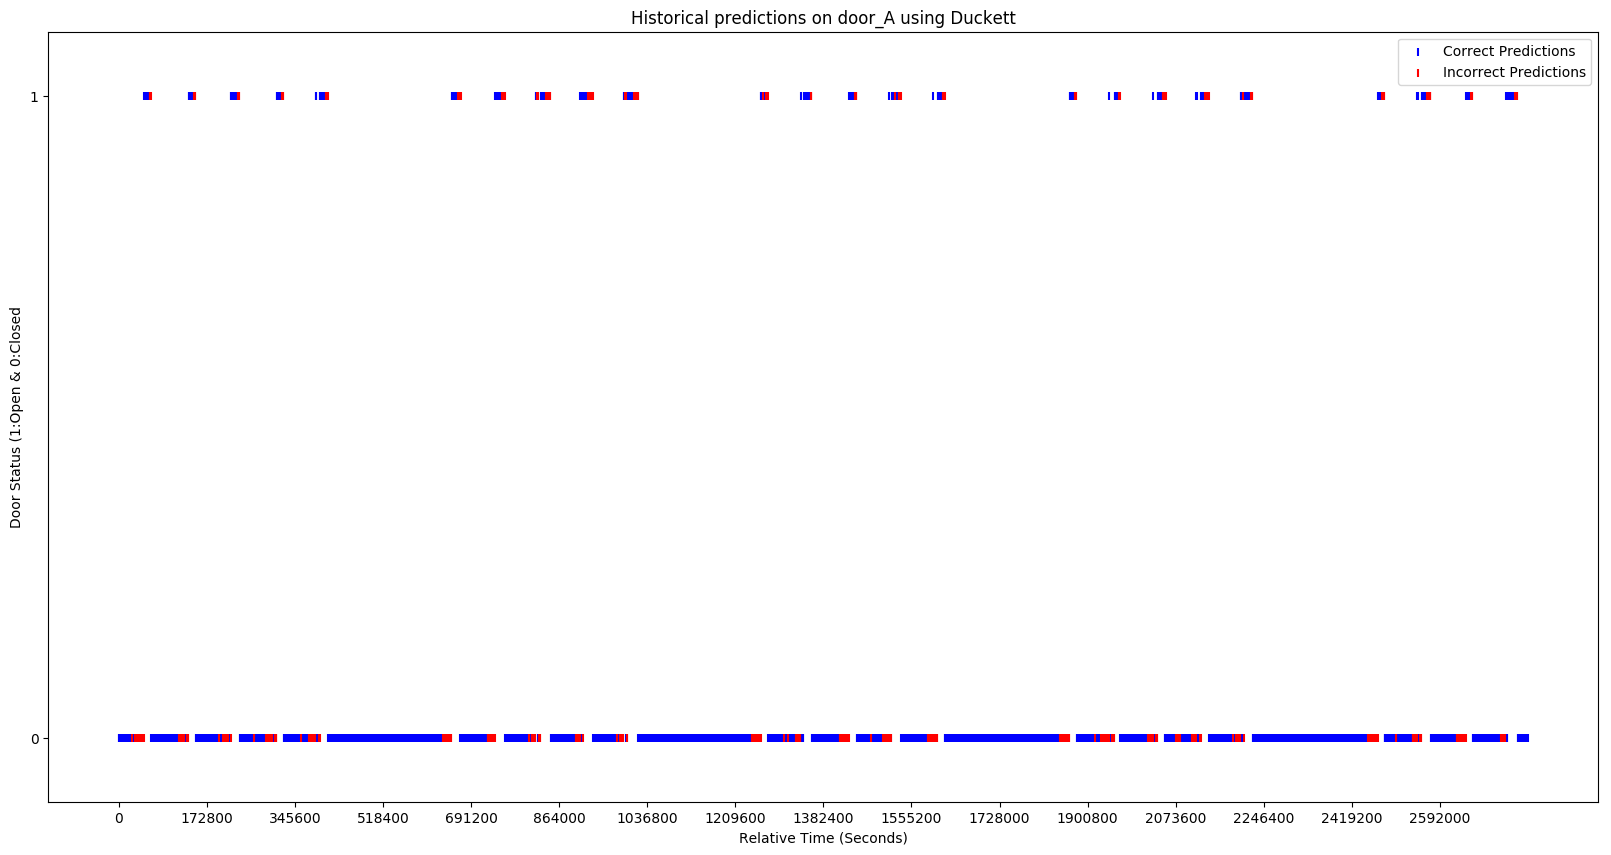
\includegraphics[width = 3in]{images/results/Historical_door_A_Duckett.png}} &
    {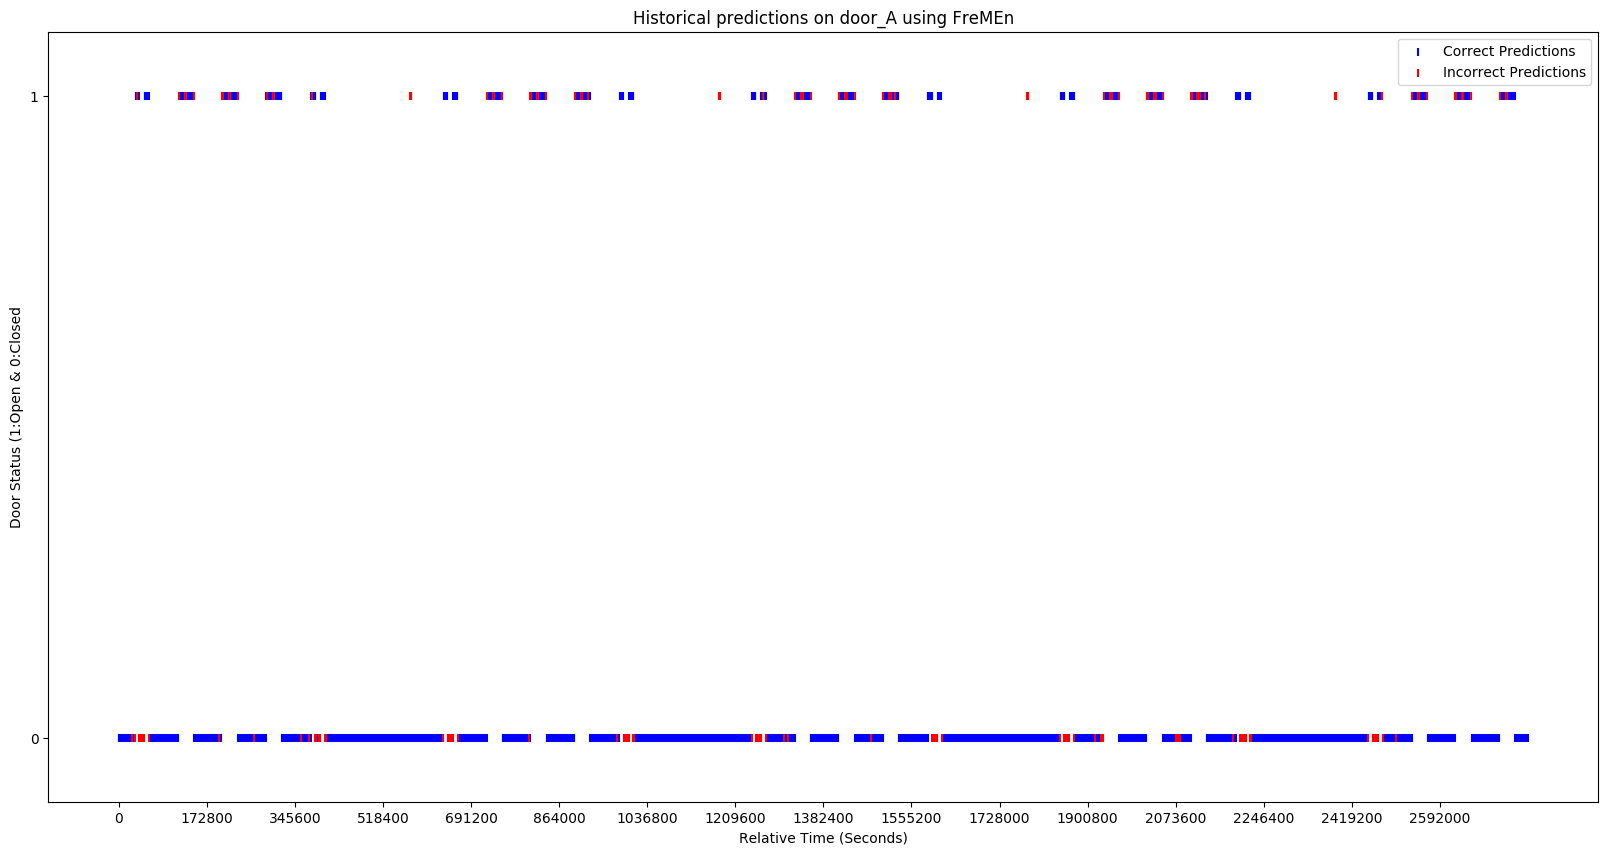
\includegraphics[width = 3in]{images/results/Historical_door_A_FreMEn.png}} \\
    {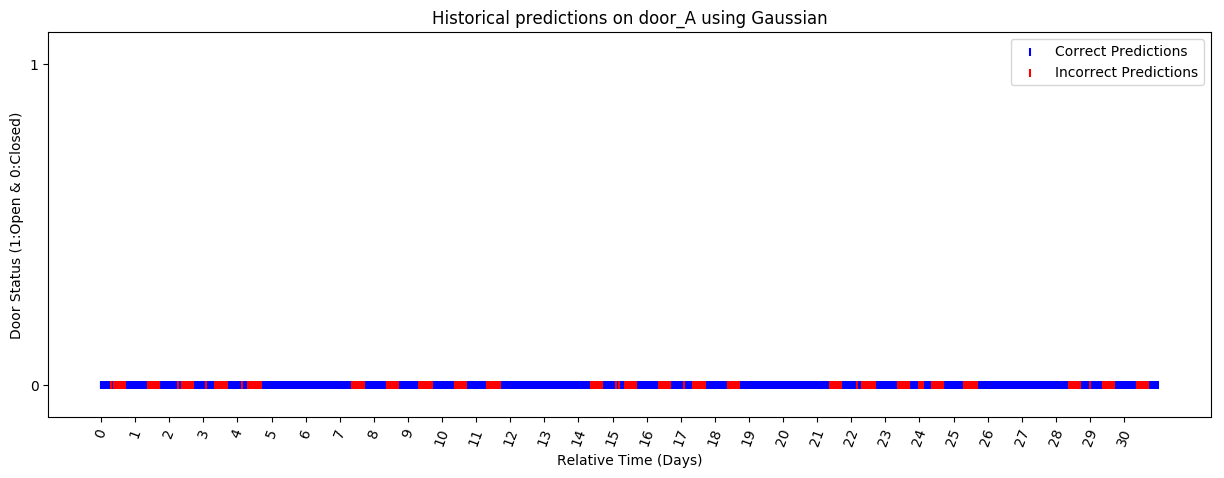
\includegraphics[width = 3in]{images/results/Historical_door_A_Gaussian.png}} &
    {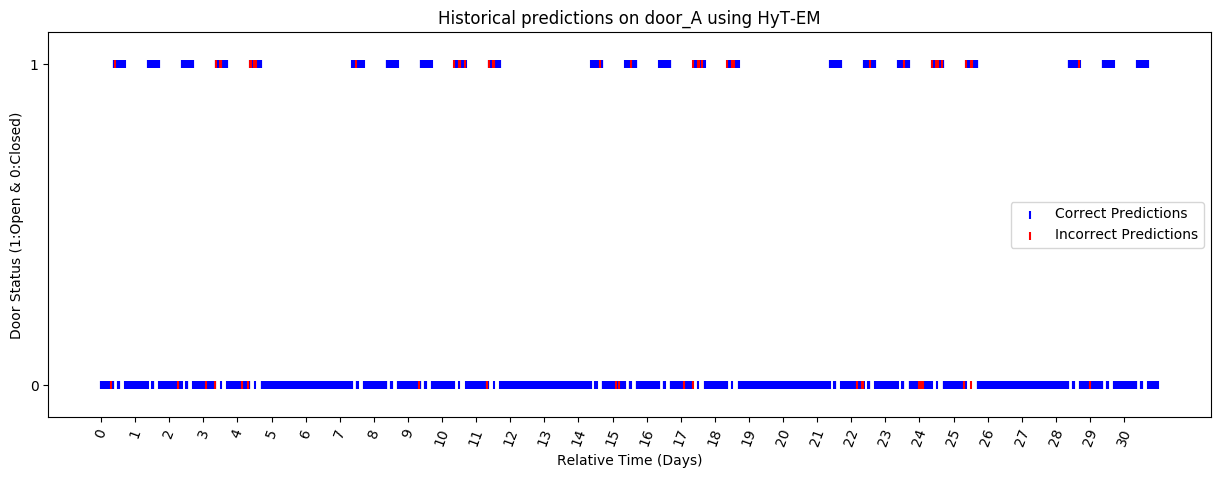
\includegraphics[width = 3in]{images/results/Historical_door_A_HyT-EM.png}} \\
  \end{tabular}
  \caption{Historical Recreations - Door A}
\end{figure} \\ \\

\begin{figure}
  \begin{tabular}{cc}
    {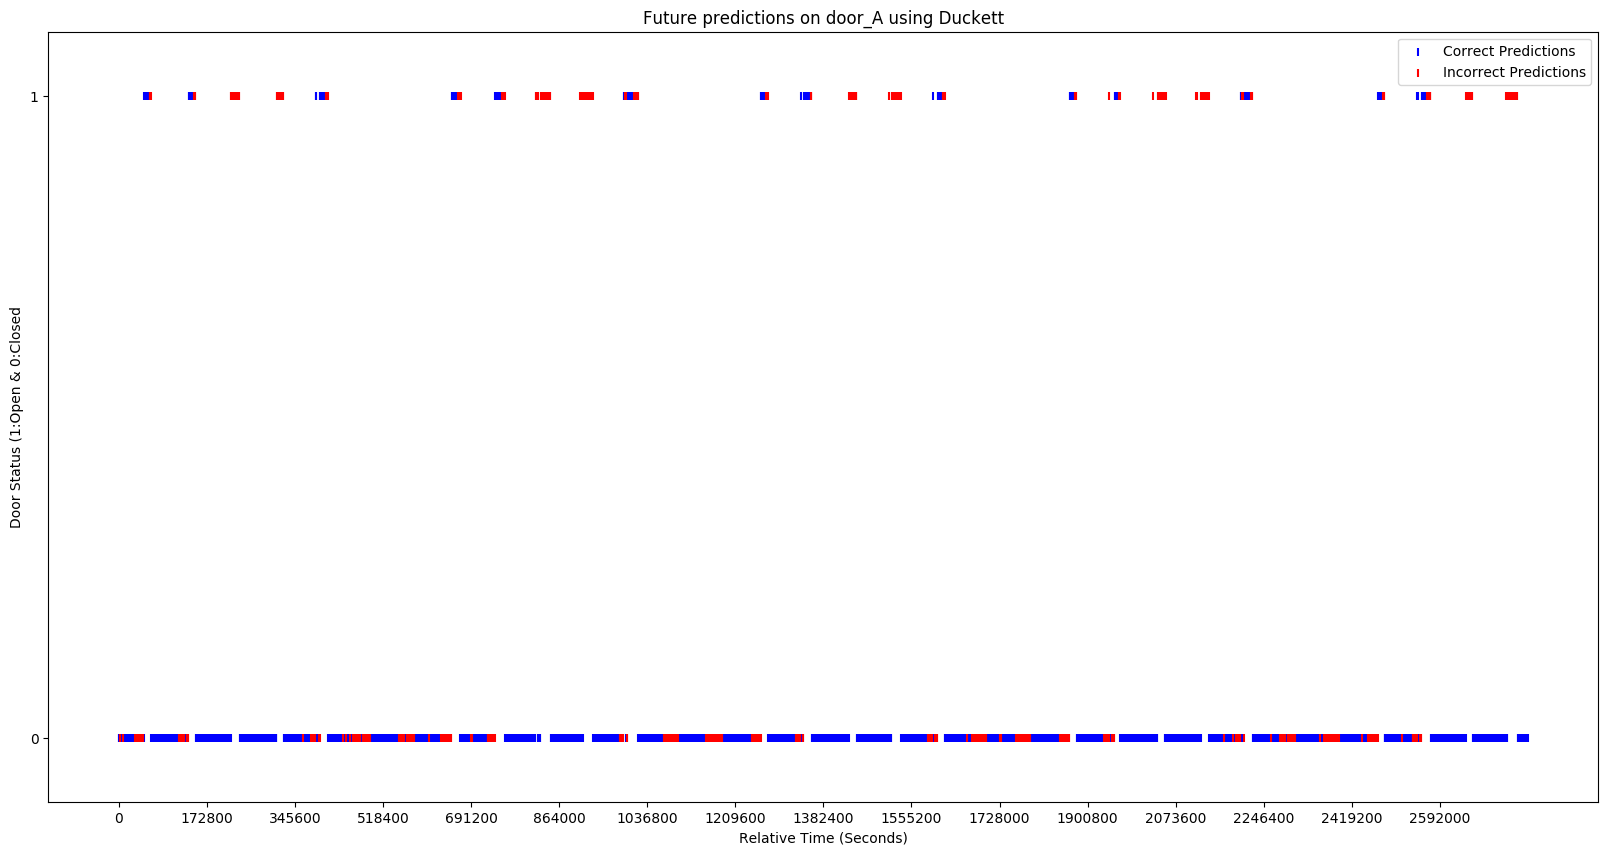
\includegraphics[width = 3in]{images/results/Future_door_A_Duckett.png}} &
    {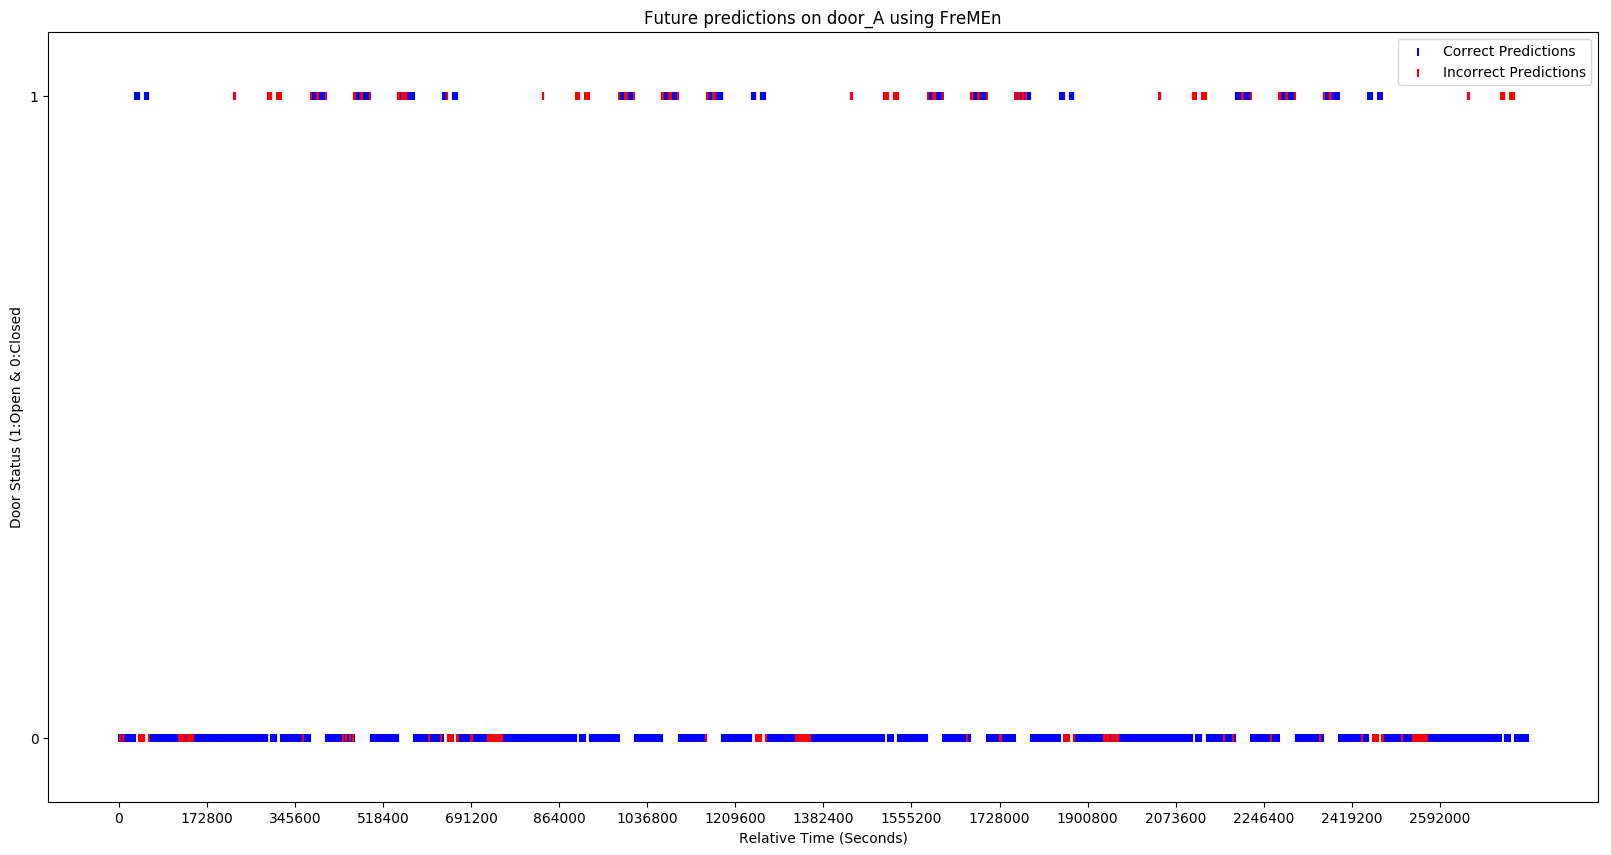
\includegraphics[width = 3in]{images/results/Future_door_A_FreMEn.png}} \\
    {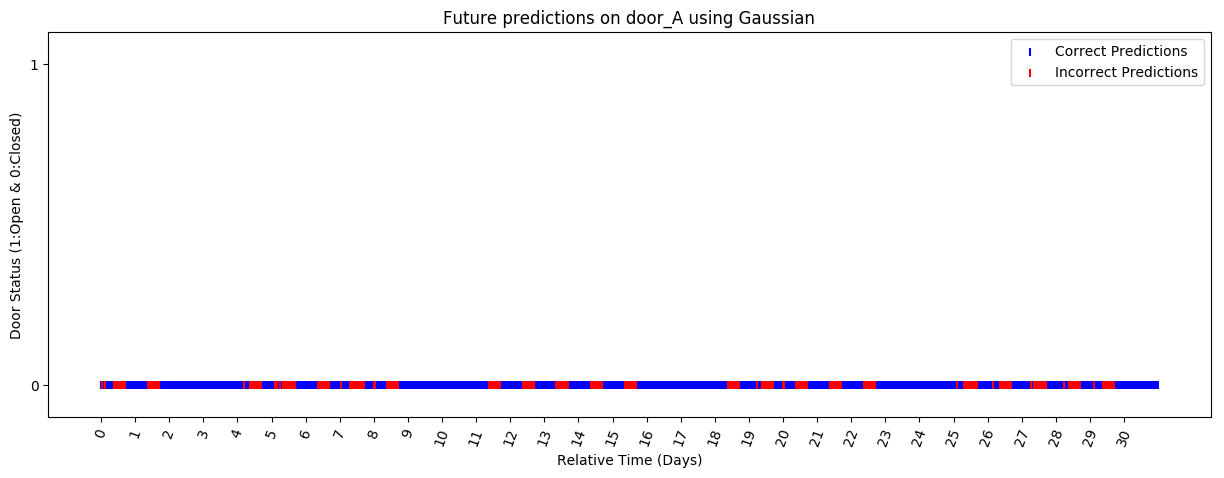
\includegraphics[width = 3in]{images/results/Future_door_A_Gaussian.png}} &
    {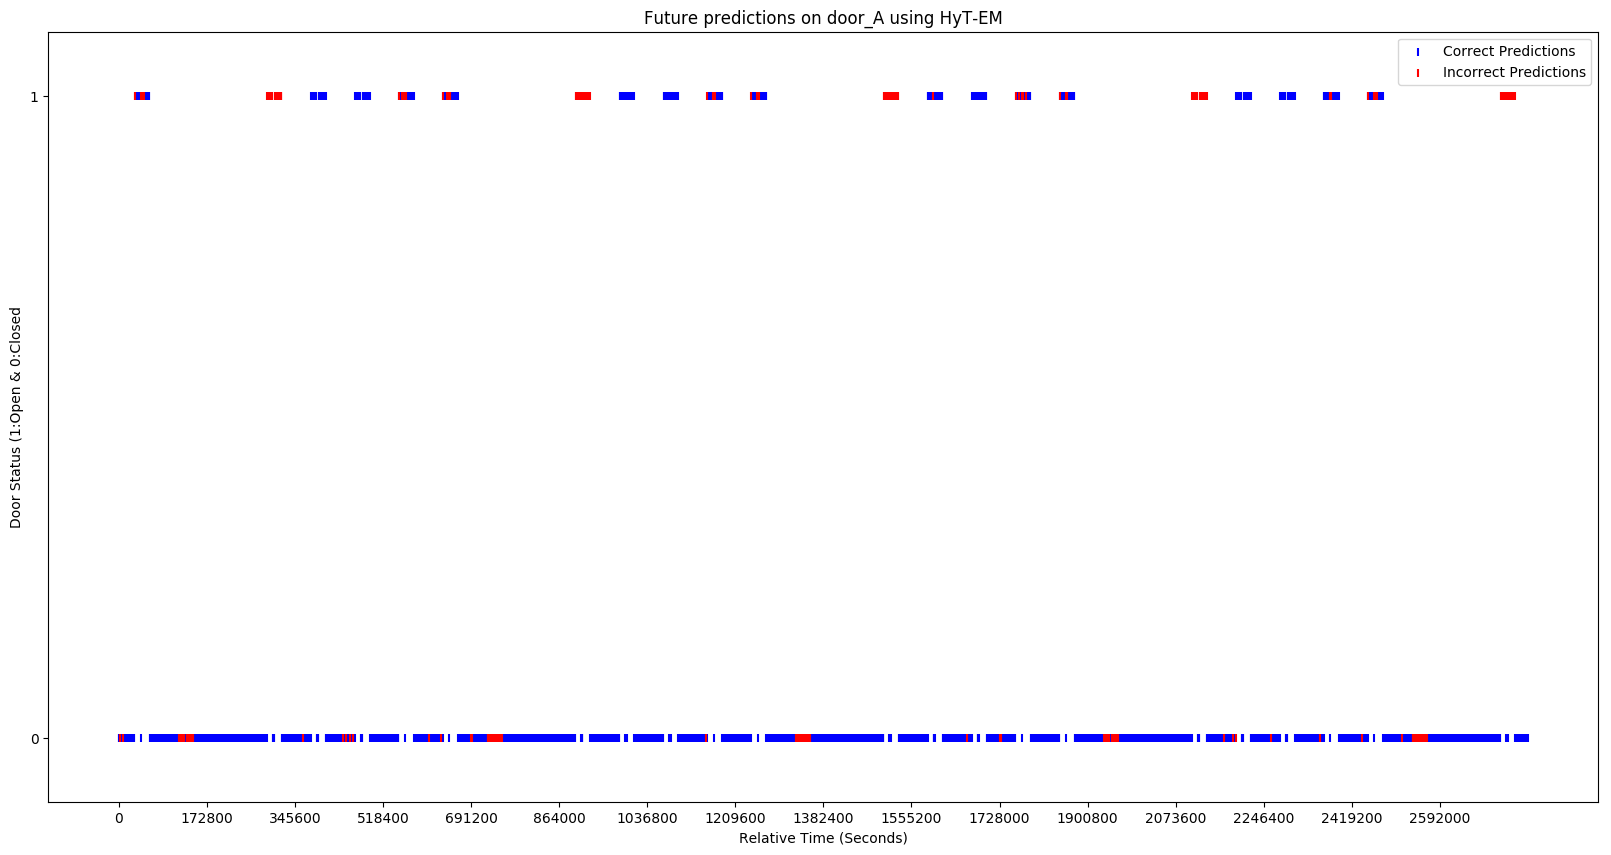
\includegraphics[width = 3in]{images/results/Future_door_A_HyT-EM.png}} \\
  \end{tabular}
  \caption{Future Predictions - Door A}
\end{figure} \\ \\

\begin{figure}
  \begin{tabular}{cc}
    {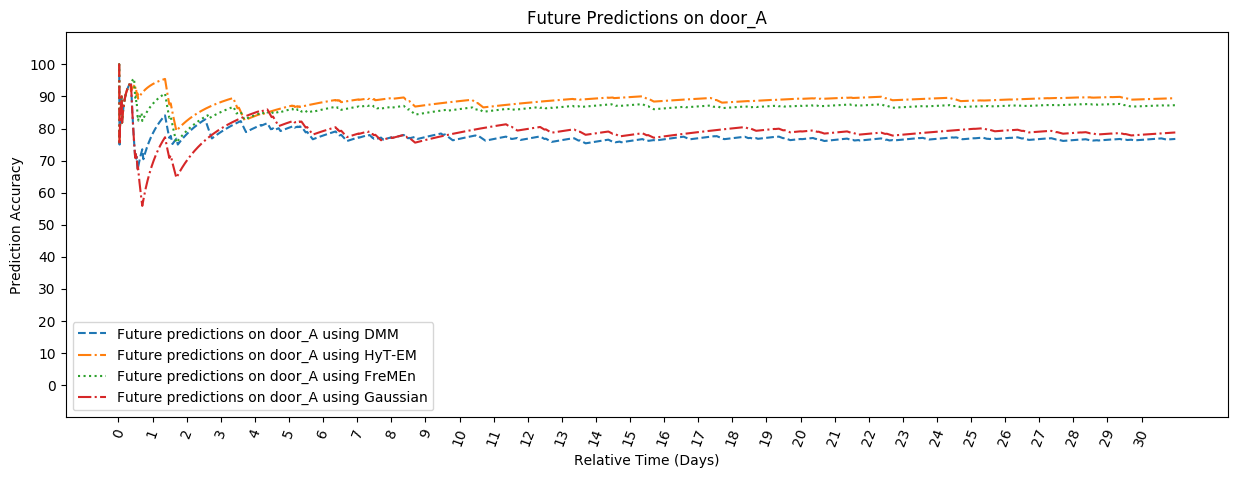
\includegraphics[width = 3in]{images/results/Future_Predictions_on_door_A.png}} &
    {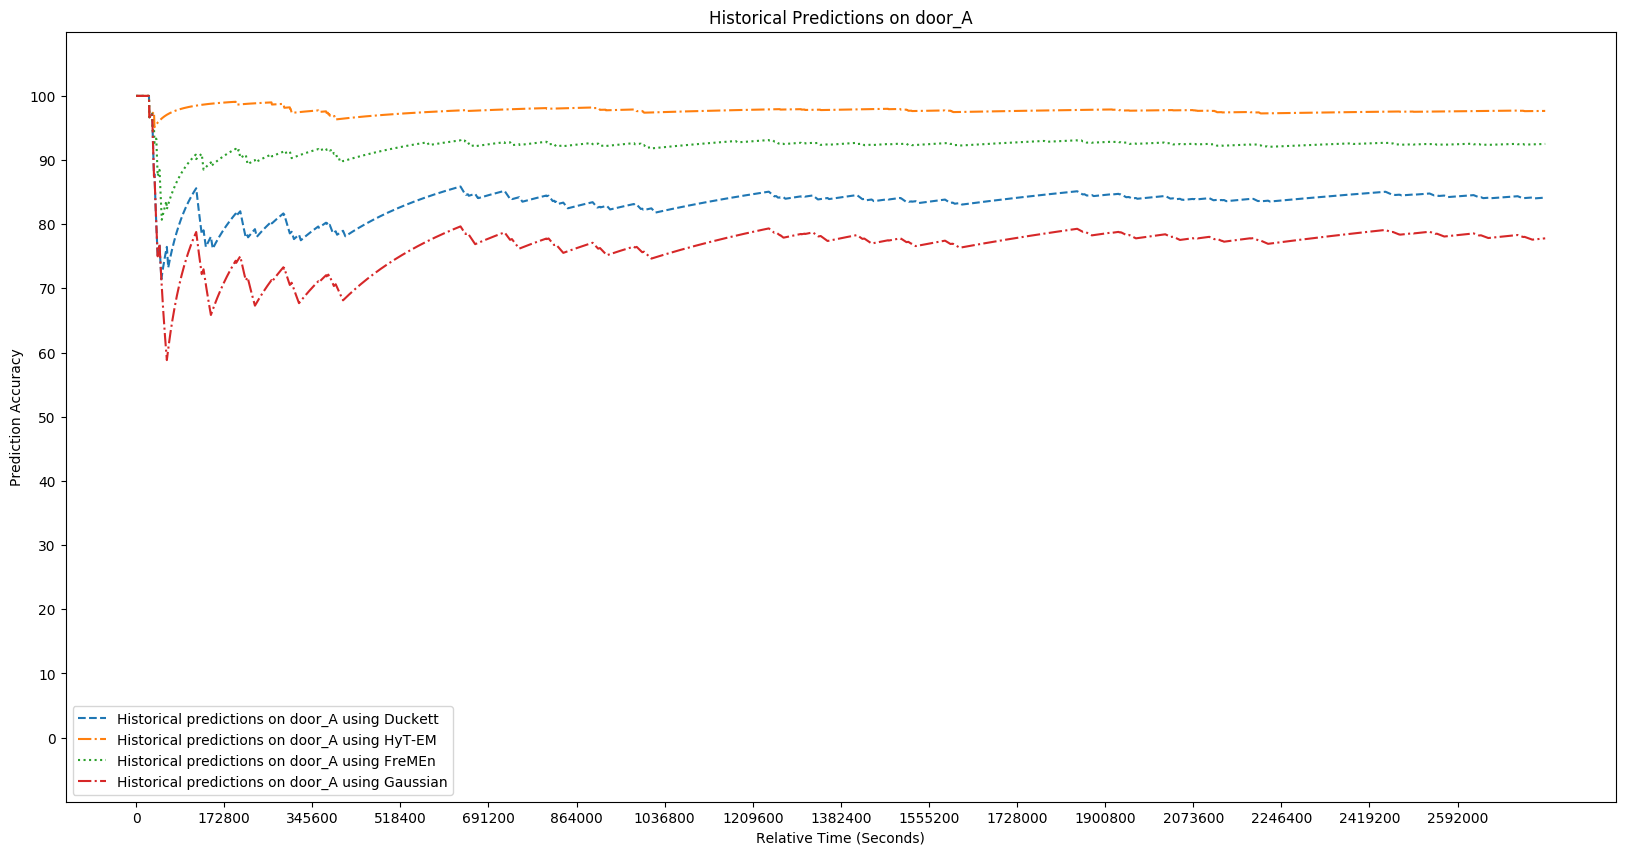
\includegraphics[width = 3in]{images/results/Historical_Predictions_on_door_A.png}} \\
  \end{tabular}
  \caption{Model Accuracy Over Time - Door A}
\end{figure} \\ \\

\subsection { Door B }

Door B demonstrates a fact the will be come increasingly clear with future
experiments.  Methods that use a modified version of the Fourier transform as
described in TODO: CITATION require a certain threshold of frequency to be met
in order to accurately predict.  In fact, it's interesting to note that the
very thing that allows these methods perform so well with periodic behavior
causes issues with datasets with non periodic behavior or datasets with
minimal periods of periodic data. \\

\begin{table}[h!]
  \centering
  \resizebox{\textwidth}{!}{%
    \begin{tabular}{|l|l|l|l|l|}
      \hline
      & Duckett & Gaussian & FreMEn  & HyperTime \\ \hline
      Historical Accuracy             & 85.71\% & 59.81\%  & 75.20\% & 71.55\%   \\ \hline
      Prediction Accuracy             & 69.24\% & 62.17\%  & 76.95\% & 75.78\%   \\ \hline
      Computation Time (Milliseconds) & 600     & 60       & 80      & 1440      \\ \hline
      Memory Usage (KB)               & 31036   & 34644    & 34892   & 37692     \\ \hline
    \end{tabular}%
  }
  \caption{Door B Data Overview}
\end{table} \\

Duckett, relying almost solely on averages, does surprisingly well on this
experiment beating out all other models in both historical and prediction
accuracy.  It is, however, important to note the flaws in Duckett's long-term
prediction. Due to the fact that future predictions are not directly possible
using Duckett and thus previous month data is used, it is clear to see that
while Duckett performed overall well historically, it is not without problems
in future prediction.  Of particular interest is its failure to continue to
accurately predict a periodic behavior that does not occur on month
boundaries. Since the behavior that happens every three days does not happen
on the same day between the two months Duckett incorrectly predicts its
occurrence as happening on the same days as last month.

In terms of resource usage, a similar trend to door A is observed. Gaussian
and FreMEn predictions take under 100 milliseconds while Duckett takes around
an order of magnitude longer, and HyperTime yet another order of magnitude
longer. Finally, similar to door A, all approaches use about the same amount
of memory for training and predicting within about 10 megabytes.

\begin{figure}
  \begin{tabular}{cc}
    {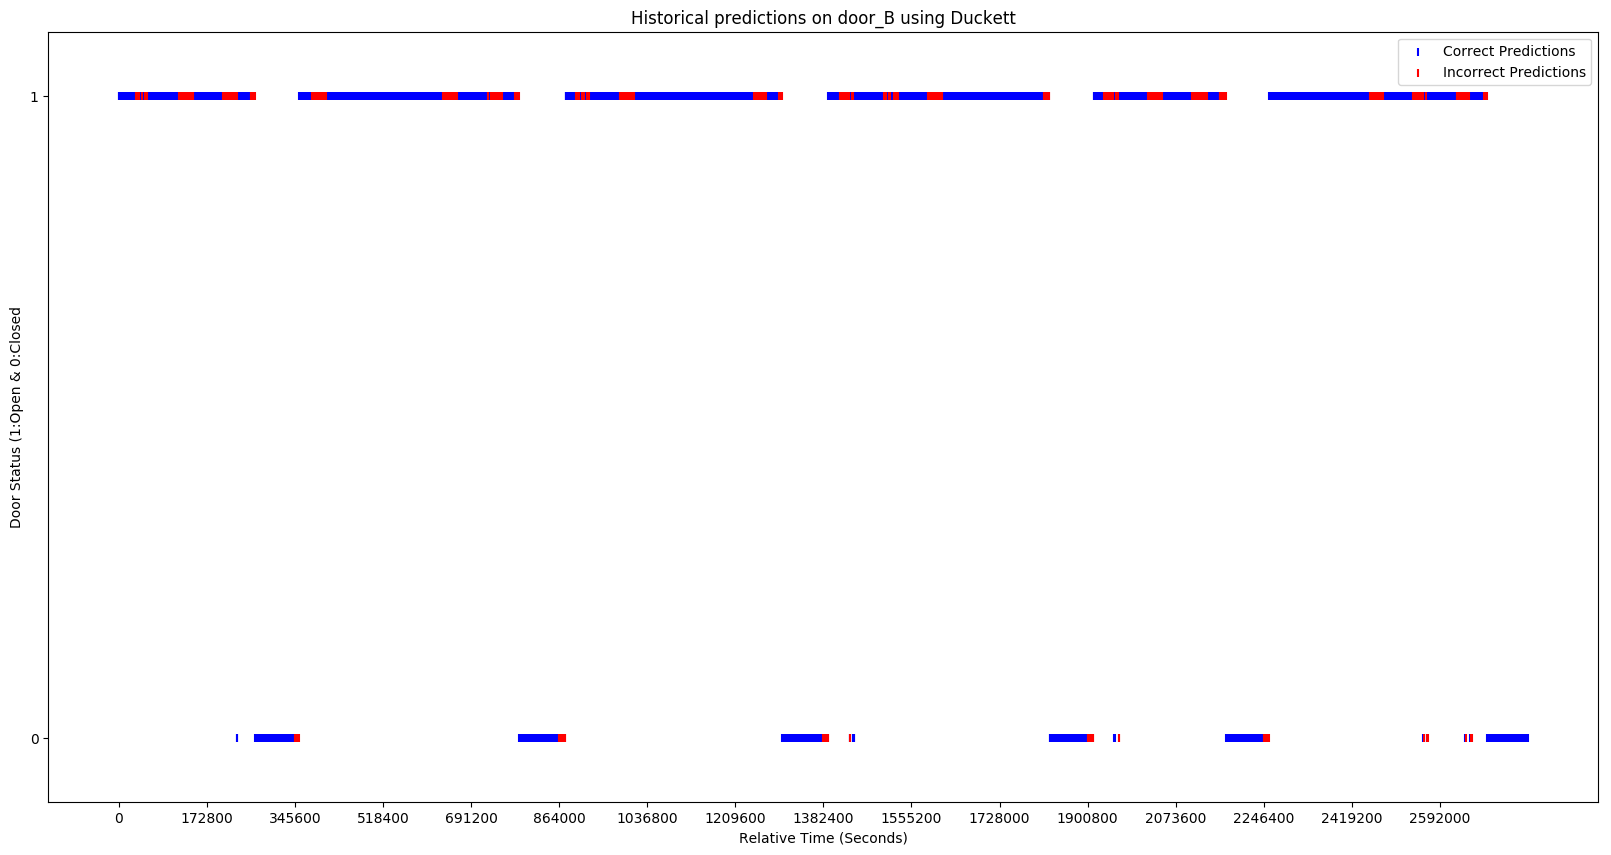
\includegraphics[width = 3in]{images/results/Historical_door_B_Duckett.png}} &
    {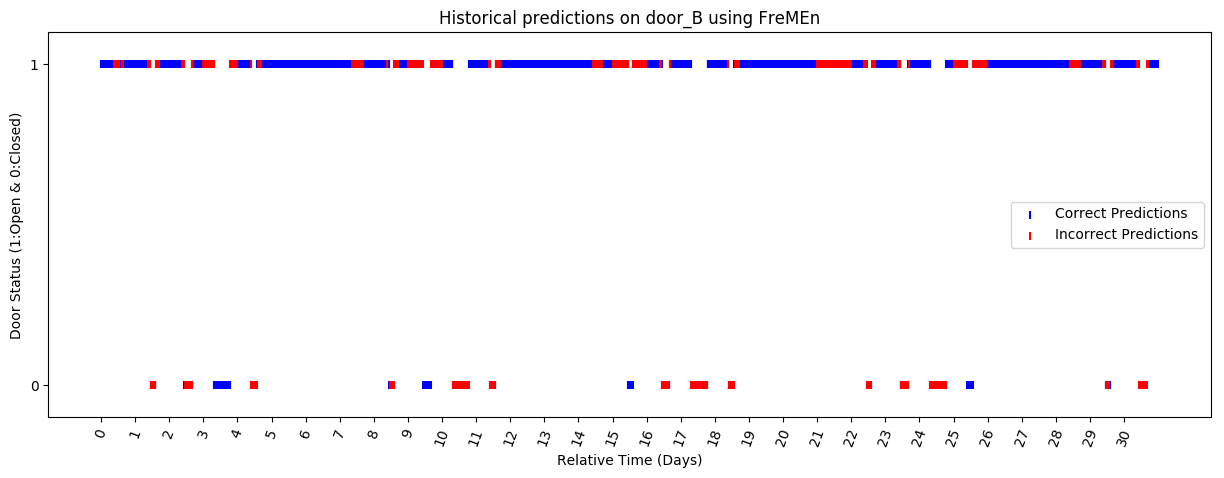
\includegraphics[width = 3in]{images/results/Historical_door_B_FreMEn.png}} \\
    {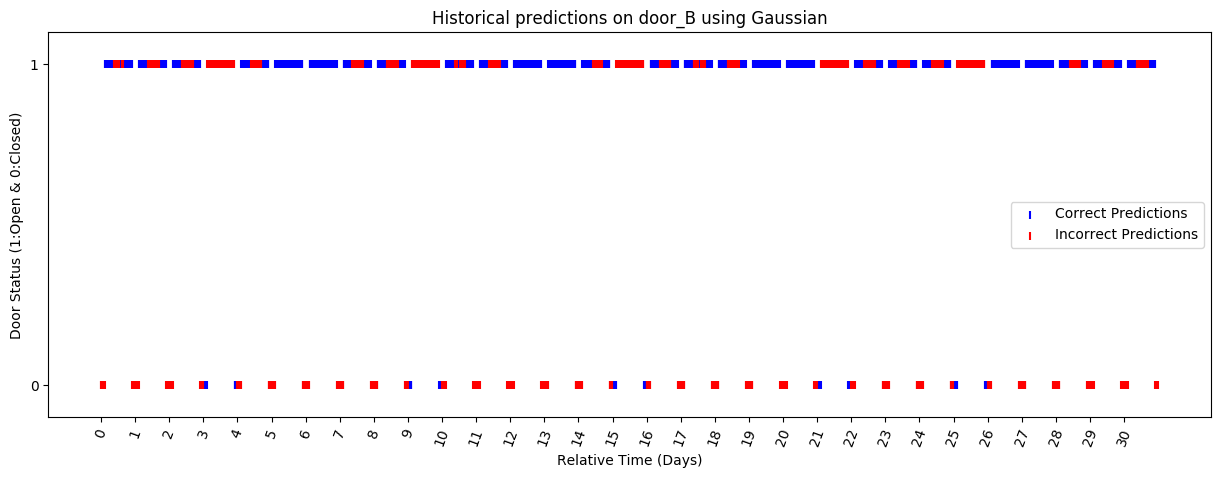
\includegraphics[width = 3in]{images/results/Historical_door_B_Gaussian.png}} &
    {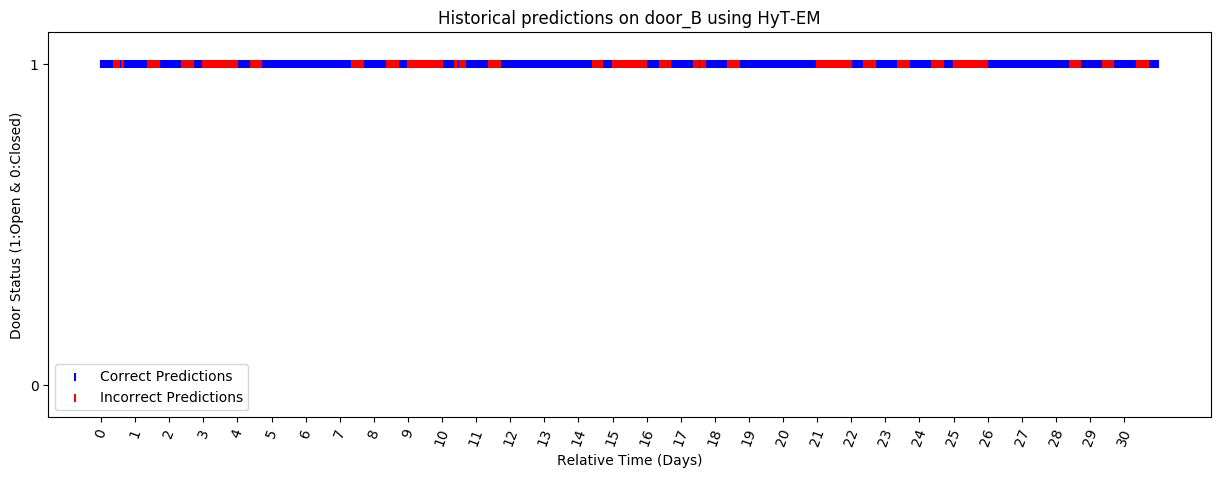
\includegraphics[width = 3in]{images/results/Historical_door_B_HyT-EM.png}} \\
  \end{tabular}
  \caption{Historical Recreations - Door B}
\end{figure}\\ \\

\begin{figure}
  \begin{tabular}{cc}
    {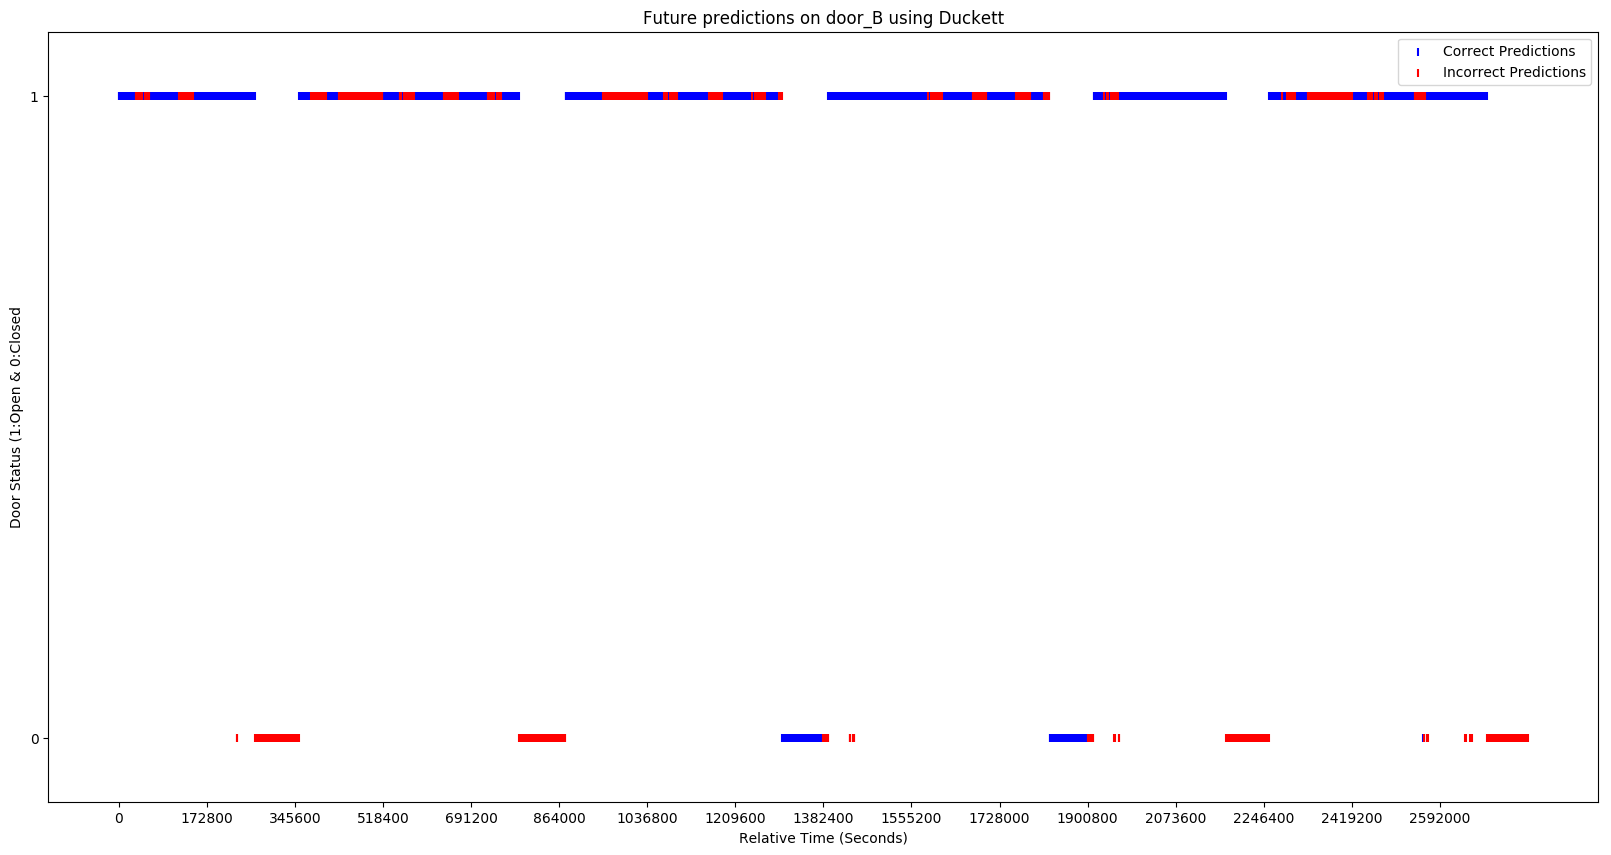
\includegraphics[width = 3in]{images/results/Future_door_B_Duckett.png}} &
    {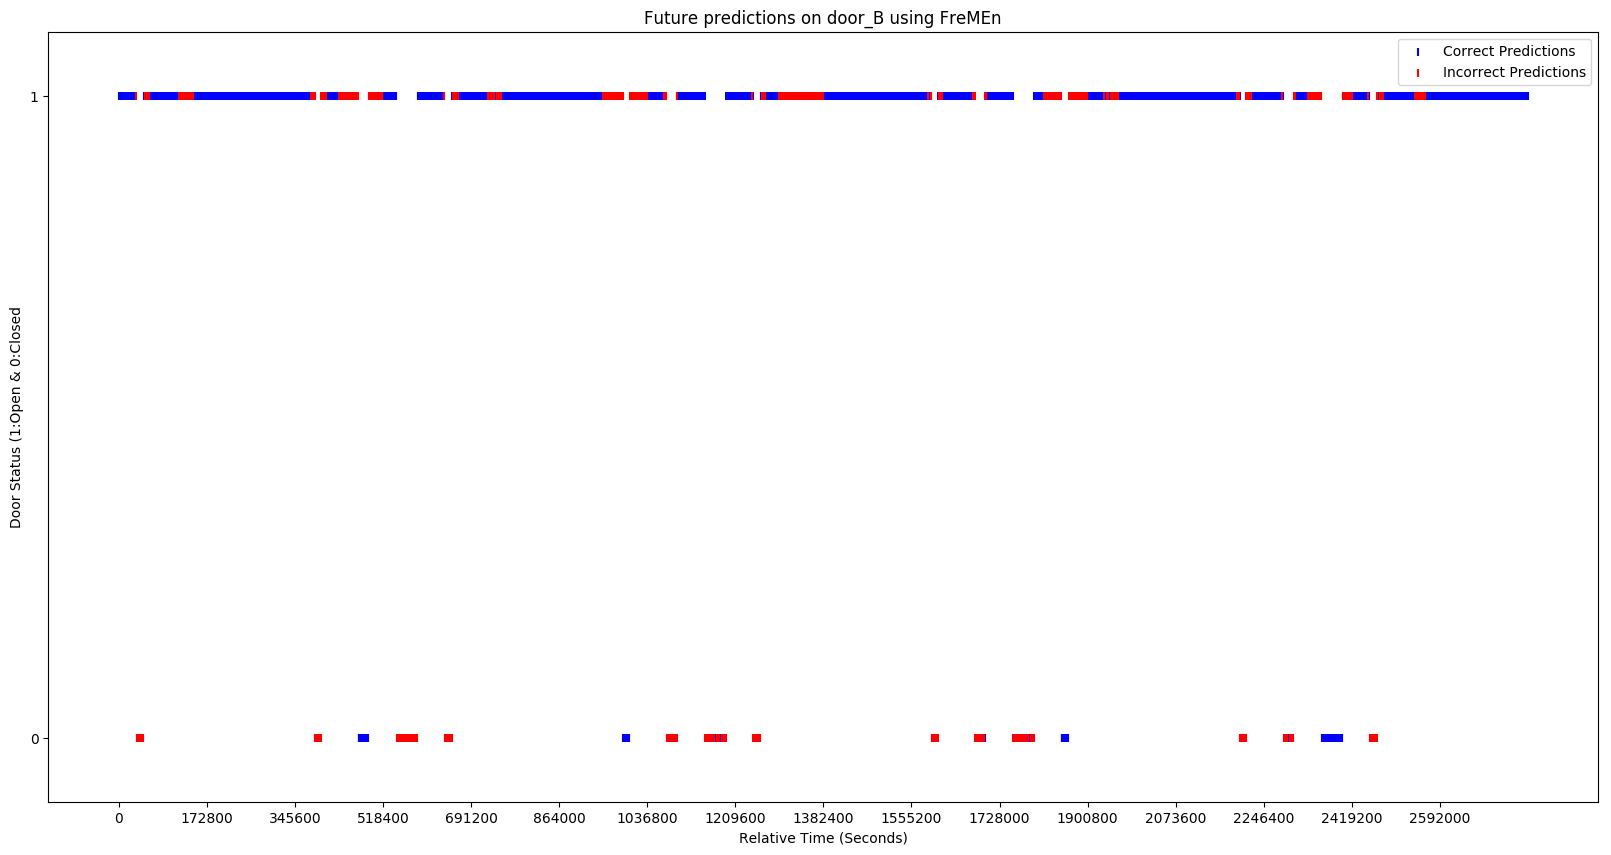
\includegraphics[width = 3in]{images/results/Future_door_B_FreMEn.png}} \\
    {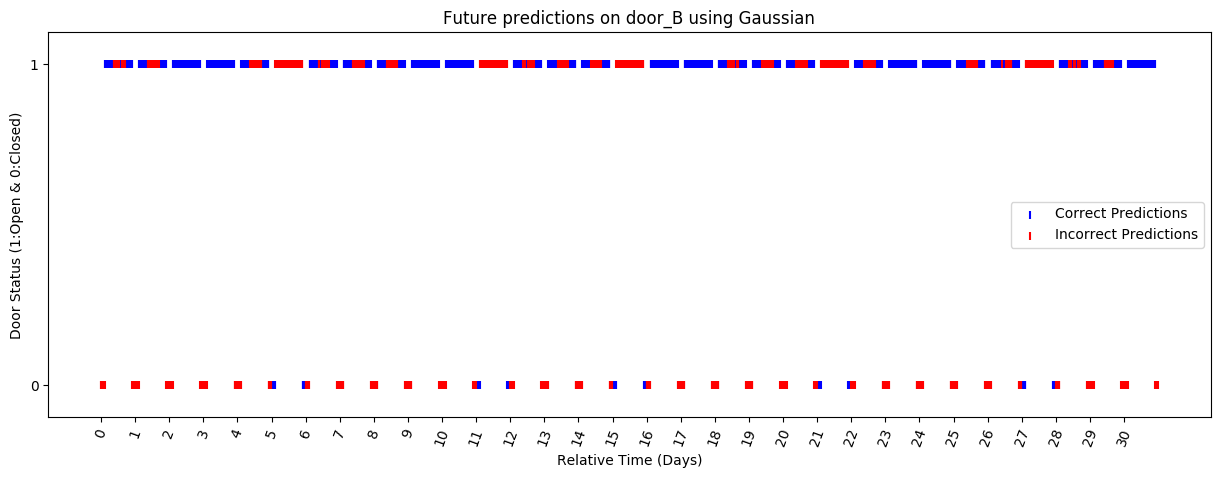
\includegraphics[width = 3in]{images/results/Future_door_B_Gaussian.png}} &
    {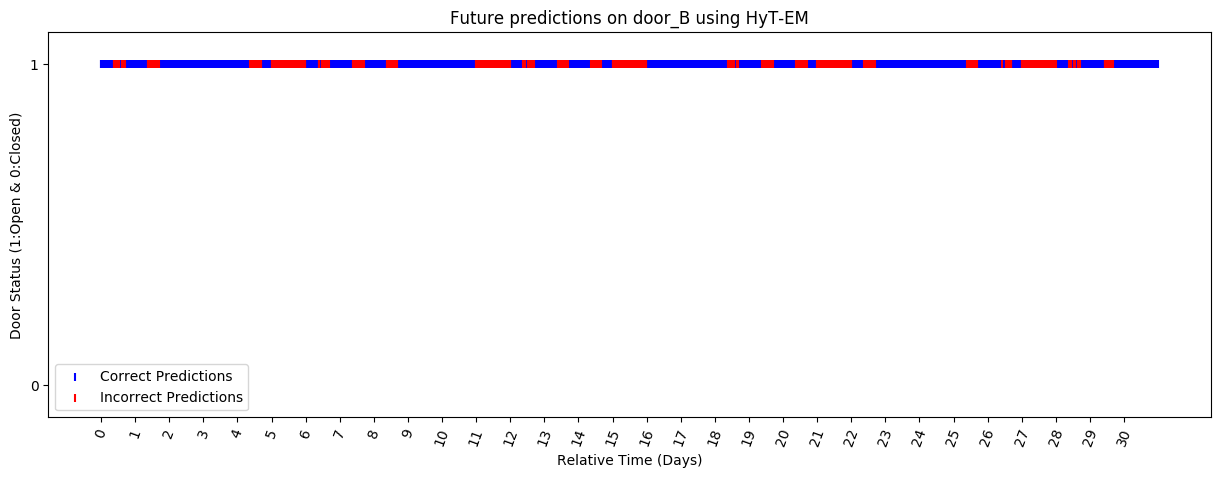
\includegraphics[width = 3in]{images/results/Future_door_B_HyT-EM.png}} \\
  \end{tabular}
  \caption{Future Predictions - Door B}
\end{figure}\\ \\

\begin{figure}
  \begin{tabular}{cc}
    {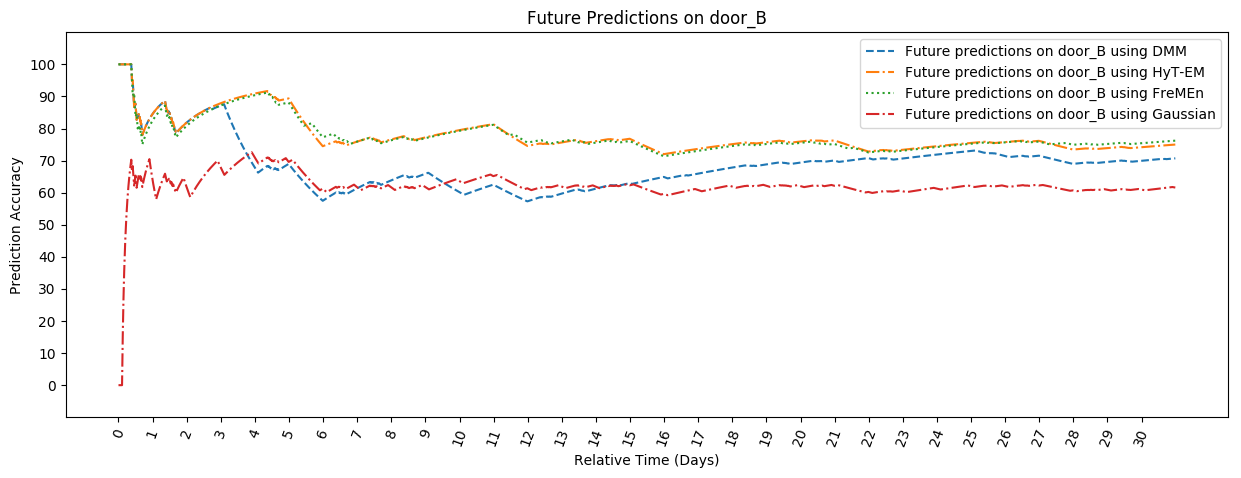
\includegraphics[width = 3in]{images/results/Future_Predictions_on_door_B.png}} &
    {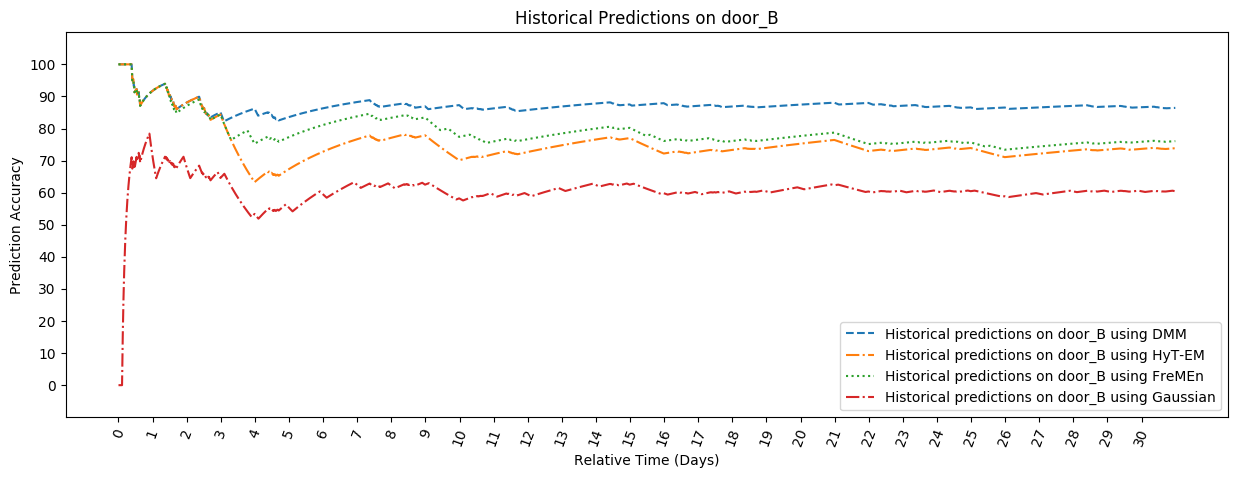
\includegraphics[width = 3in]{images/results/Historical_Predictions_on_door_B.png}} \\
  \end{tabular}
  \caption{Model Accuracy Over Time - Door B}
\end{figure}\\ \\



\subsection { Door C }

With door A exemplifying the occasionally periodic and somewhat noisy
behaviour in the real world, door C serves as almost the exact opposite,
modeling a one time, long-term change.
Perhaps some what expectedly, the results in terms of prediction accuracy are
almost completely opposite that of door A with Duckett having the best
performance both historically and with future predictions. \\

Unfortunately, despite its better performance by the numbers in table 6.3,
looking at the resulting graphs in table 6.7 and 6.8 shows a somewhat
initially disappointing result. As discussed in the door B experiment,
Duckett, merely uses it's historically prediction again for future
predictions. This is clearly visible by the prediction of the door being open
for the first three weeks in the future predictions.  However, Duckett was not
designed for long-term future predictions and instead meant to be used
``live''. When this is accounted for, Duckett's performance is once again
impressive.  In fact, as discussed TODO: where will this be discussed? the
historical predictions made by Duckett can be view as it's ``live''
predictions and thus it would be expected that in the real world it would
continue to predict the door as being closed as long as long-term future
predictions are not requested. This means that it is likely Duckett's
performance would be closer to 100\% for future actives for as long as the door
remained shut. \\

\begin{table}[h!]
  \centering
  \resizebox{\textwidth}{!}{%
    \begin{tabular}{|l|l|l|l|l|}
      \hline
      & Duckett & Gaussian & FreMEn  & HyperTime \\ \hline
      Historical Accuracy             & 99.56\% & 62.75\%  & 67.74\% & 67.74\%   \\ \hline
      Prediction Accuracy             & 31.82\% & 14.58\%  & 00.00\% & 00.00\%   \\ \hline
      Computation Time (Milliseconds) & 570     & 60       & 70      & 530       \\ \hline
      Memory Usage (KB)               & 31224   & 35004    & 34976   & 37208     \\ \hline
    \end{tabular}%
  }

  \caption{Door C Data Overview}
\end{table}

As alluded to above in door B's experiment, the lack of periodic data has
caused both FreMEn and HyperTime to take the easiest prediction for the
training data and predict that the door will always be open. Unfortunately,
this causes the future predictions to be entirely inaccurate. The only possible redemption
for the Fourier based approaches on this long term changes is that the
prediction would eventually flip to always being closed, but only after the total number of observations of the door being
closed surpassed that of the door being open. In this case, that would take a
total of just over 6 weeks if training was being done every night. \\

The resource usage statistics in figure 6.3 do interestingly break slightly
from the norm. It appears that due to the simplistic predictions of the
Fourier approaches, HyperTime has shaved off an order of magnitude in
computation time. This is believed to be because the prediction model created
by HyperTime, after the initial naive approach, has a larger error than the first and thus it immediately quits
and stops attempting to improve the model. This is irrelevant however, seeing
as the predictions are completely inaccurate so any gain in computational time
is meaningless.

\begin{figure}
  \begin{tabular}{cc}
    {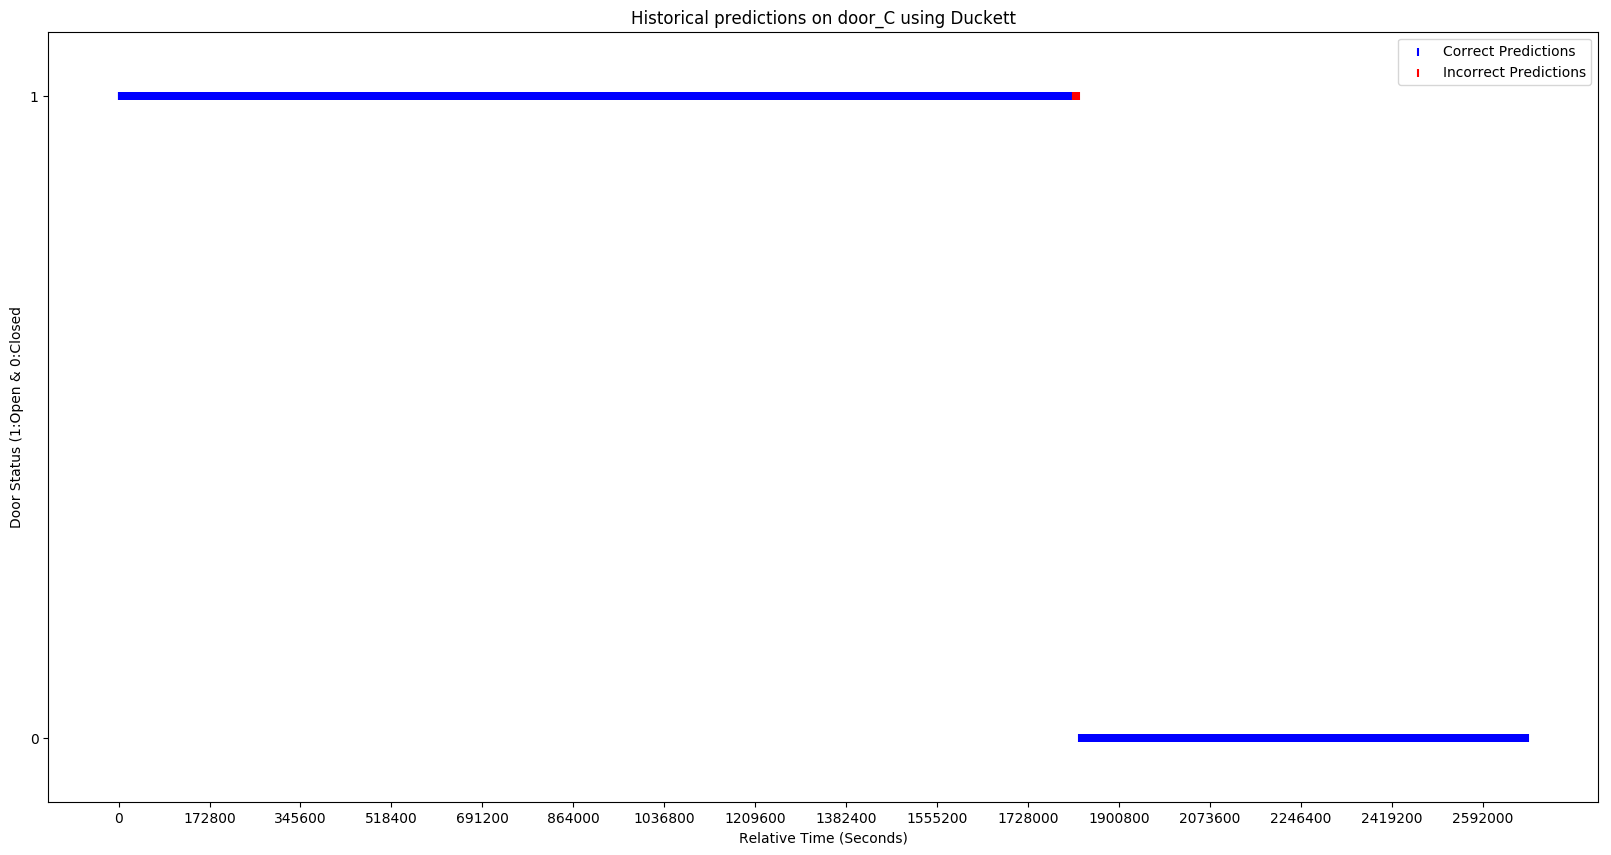
\includegraphics[width = 3in]{images/results/Historical_door_C_Duckett.png}} &
    {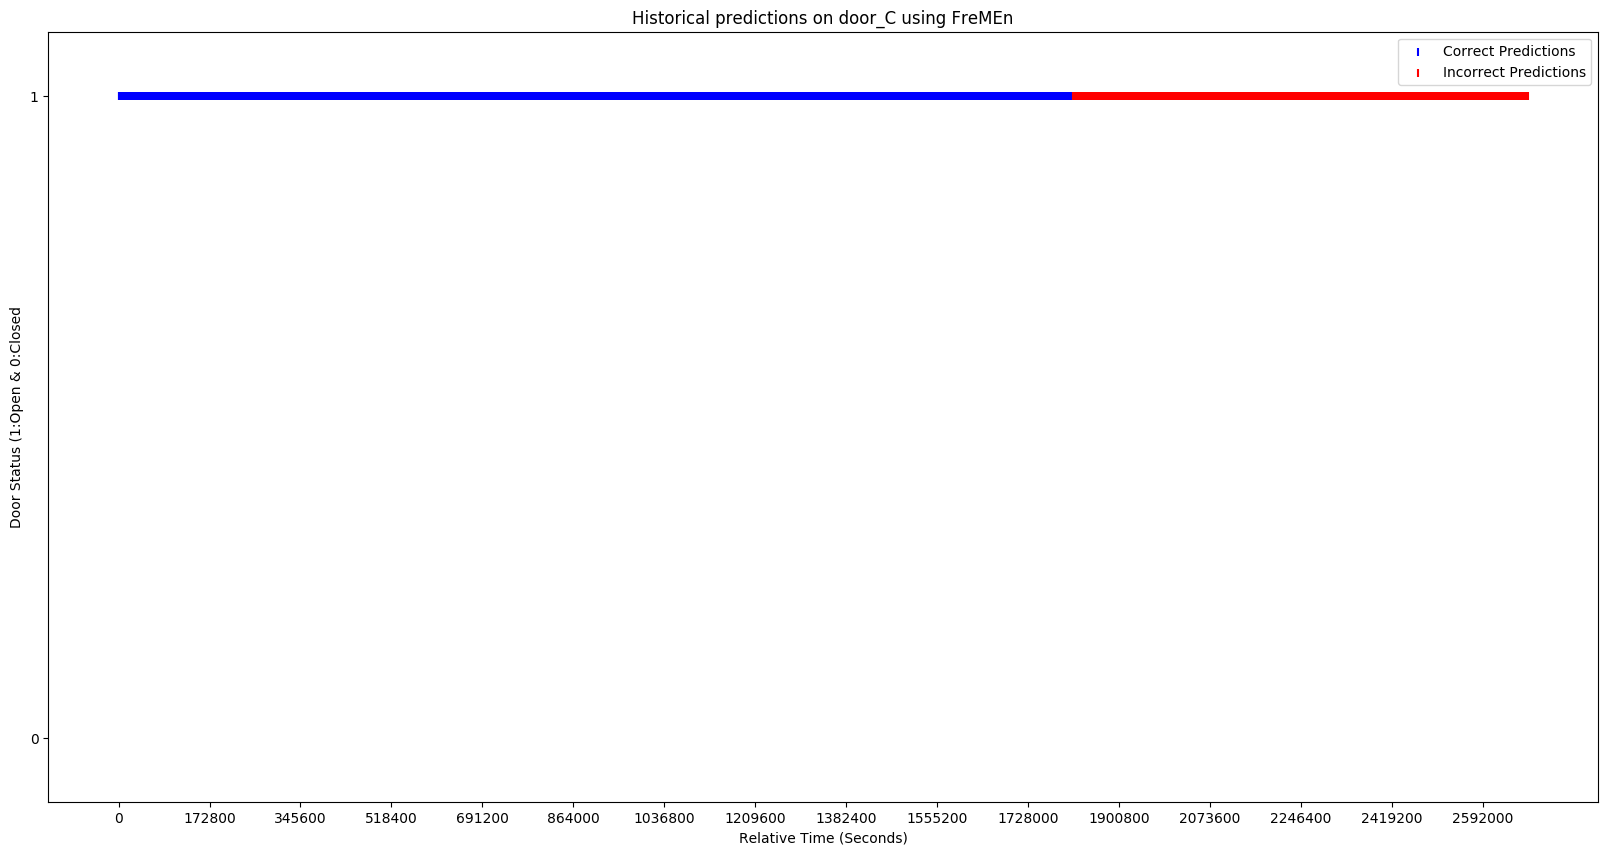
\includegraphics[width = 3in]{images/results/Historical_door_C_FreMEn.png}} \\
    {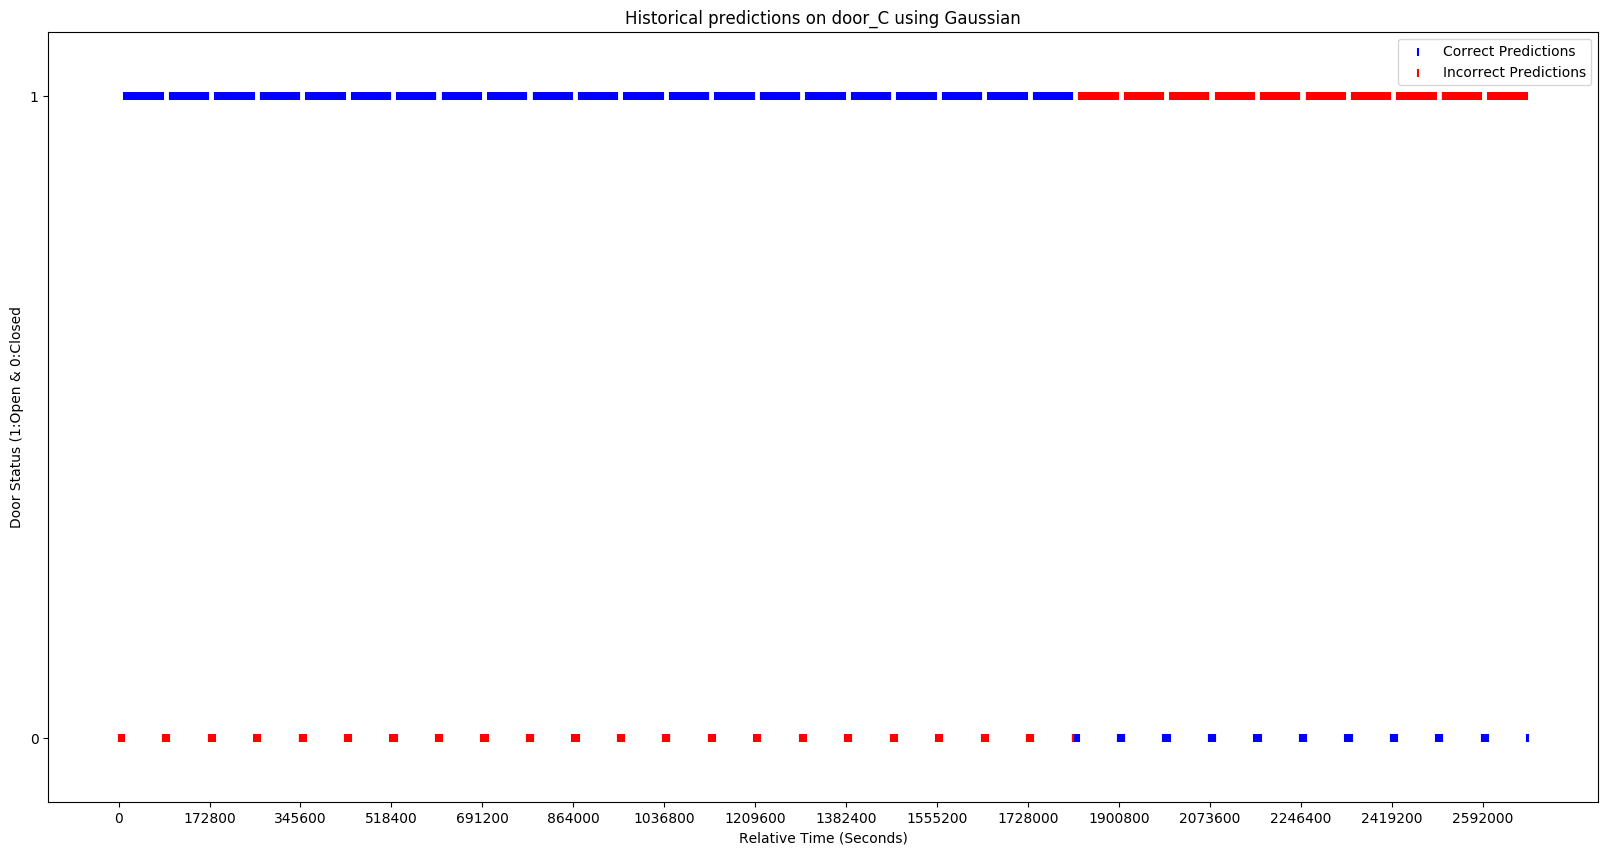
\includegraphics[width = 3in]{images/results/Historical_door_C_Gaussian.png}} &
    {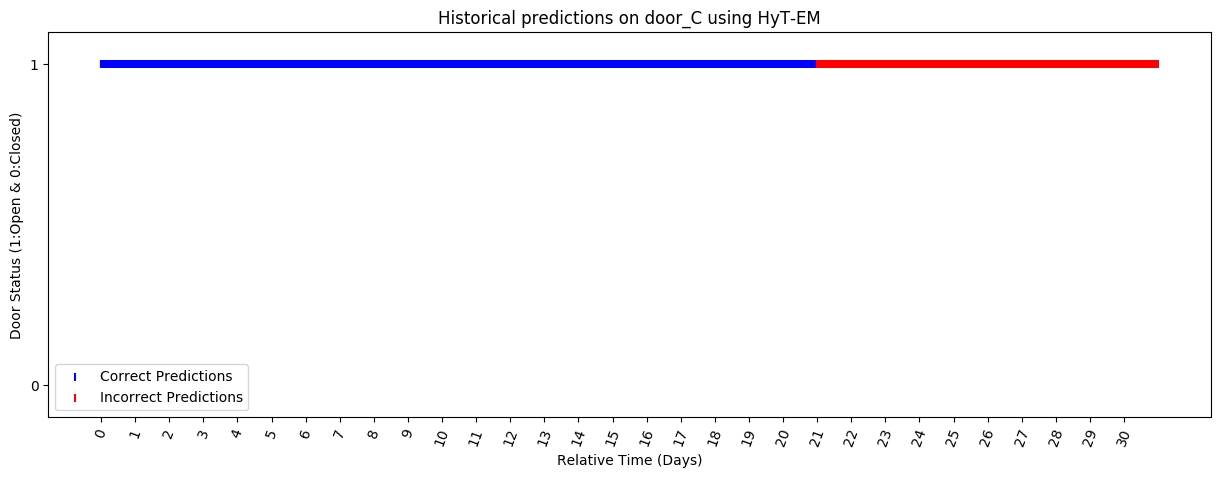
\includegraphics[width = 3in]{images/results/Historical_door_C_HyT-EM.png}} \\
  \end{tabular}
  \caption{Historical Recreations - Door C}
\end{figure}\\ \\

\begin{figure}
  \begin{tabular}{cc}
    {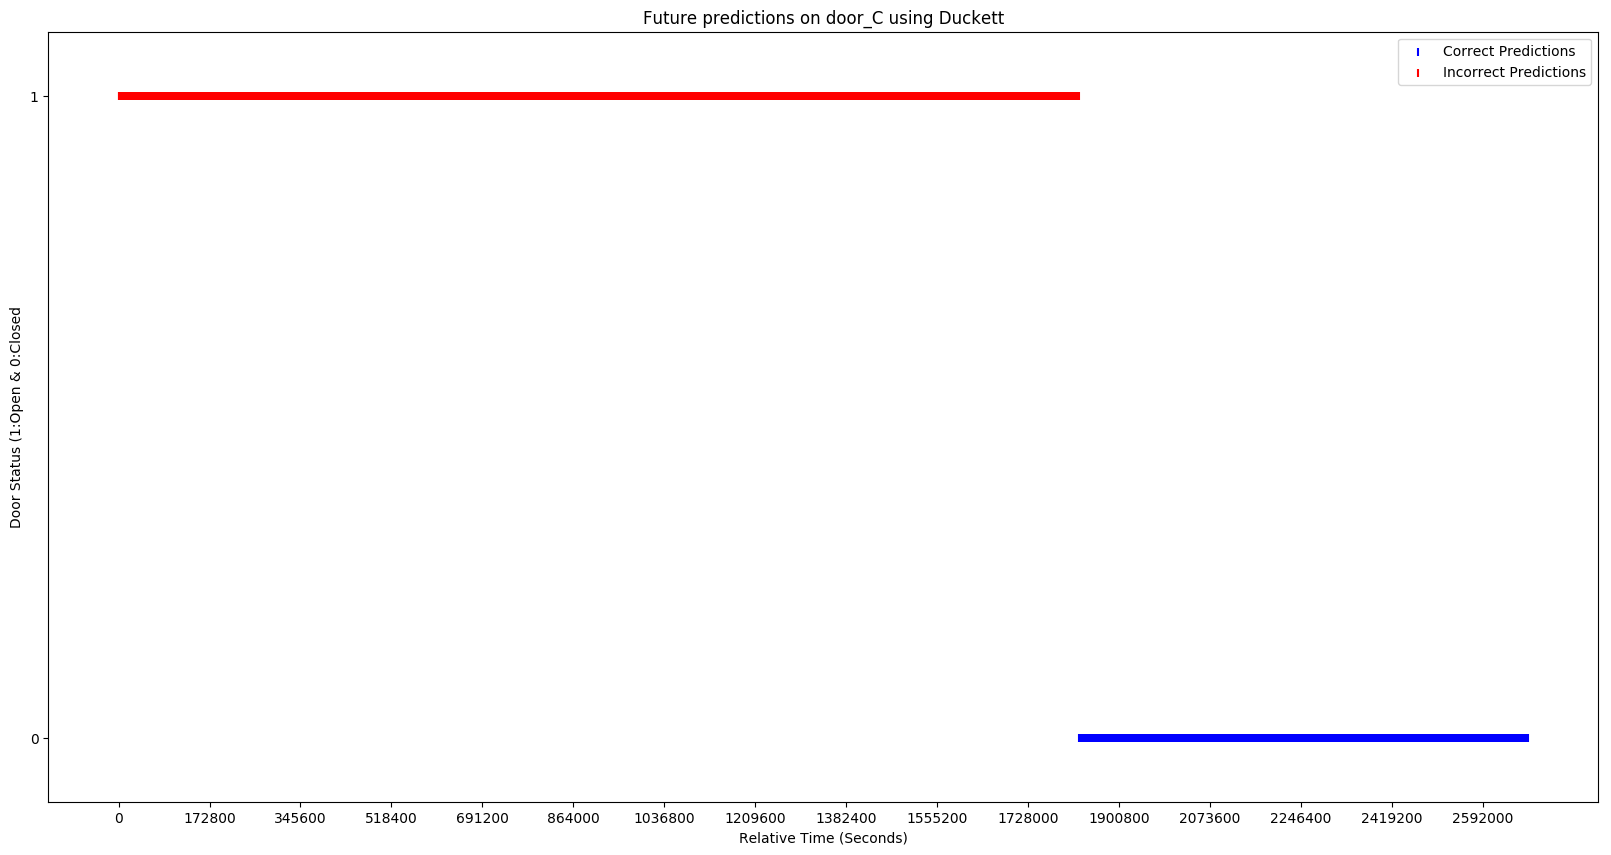
\includegraphics[width = 3in]{images/results/Future_door_C_Duckett.png}} &
    {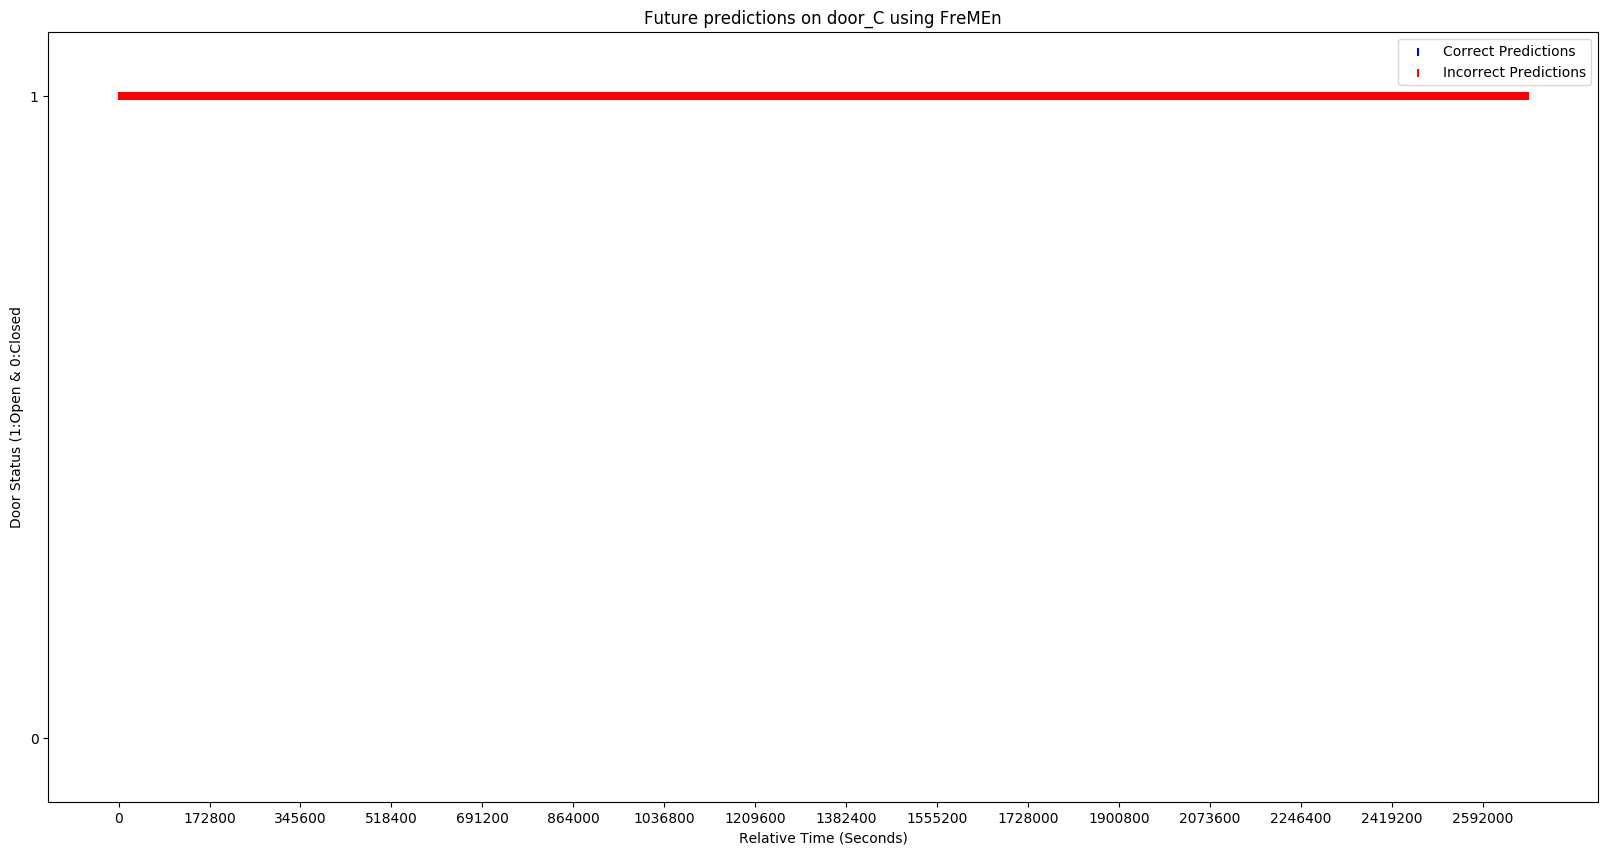
\includegraphics[width = 3in]{images/results/Future_door_C_FreMEn.png}} \\
    {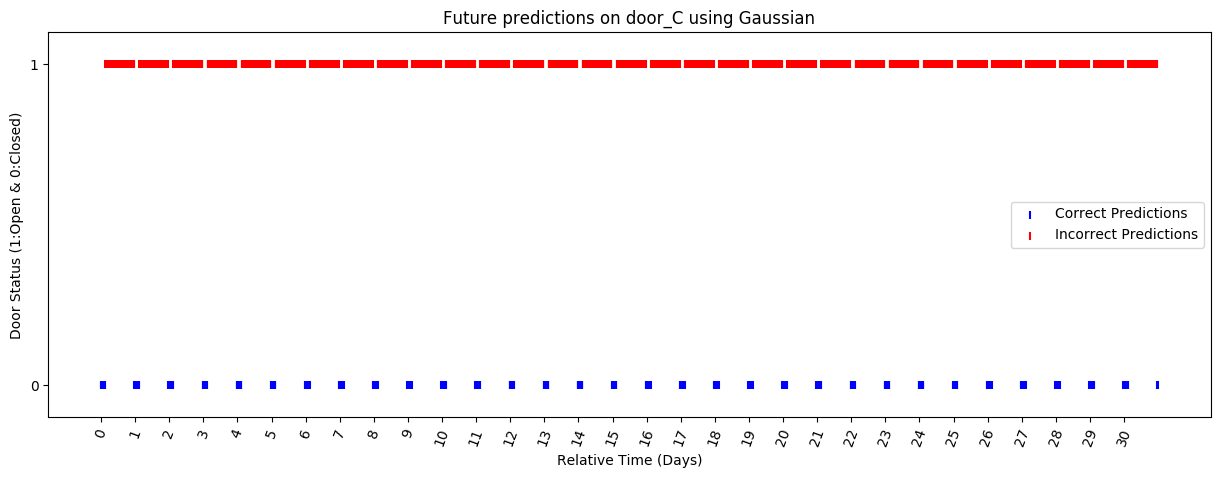
\includegraphics[width = 3in]{images/results/Future_door_C_Gaussian.png}} &
    {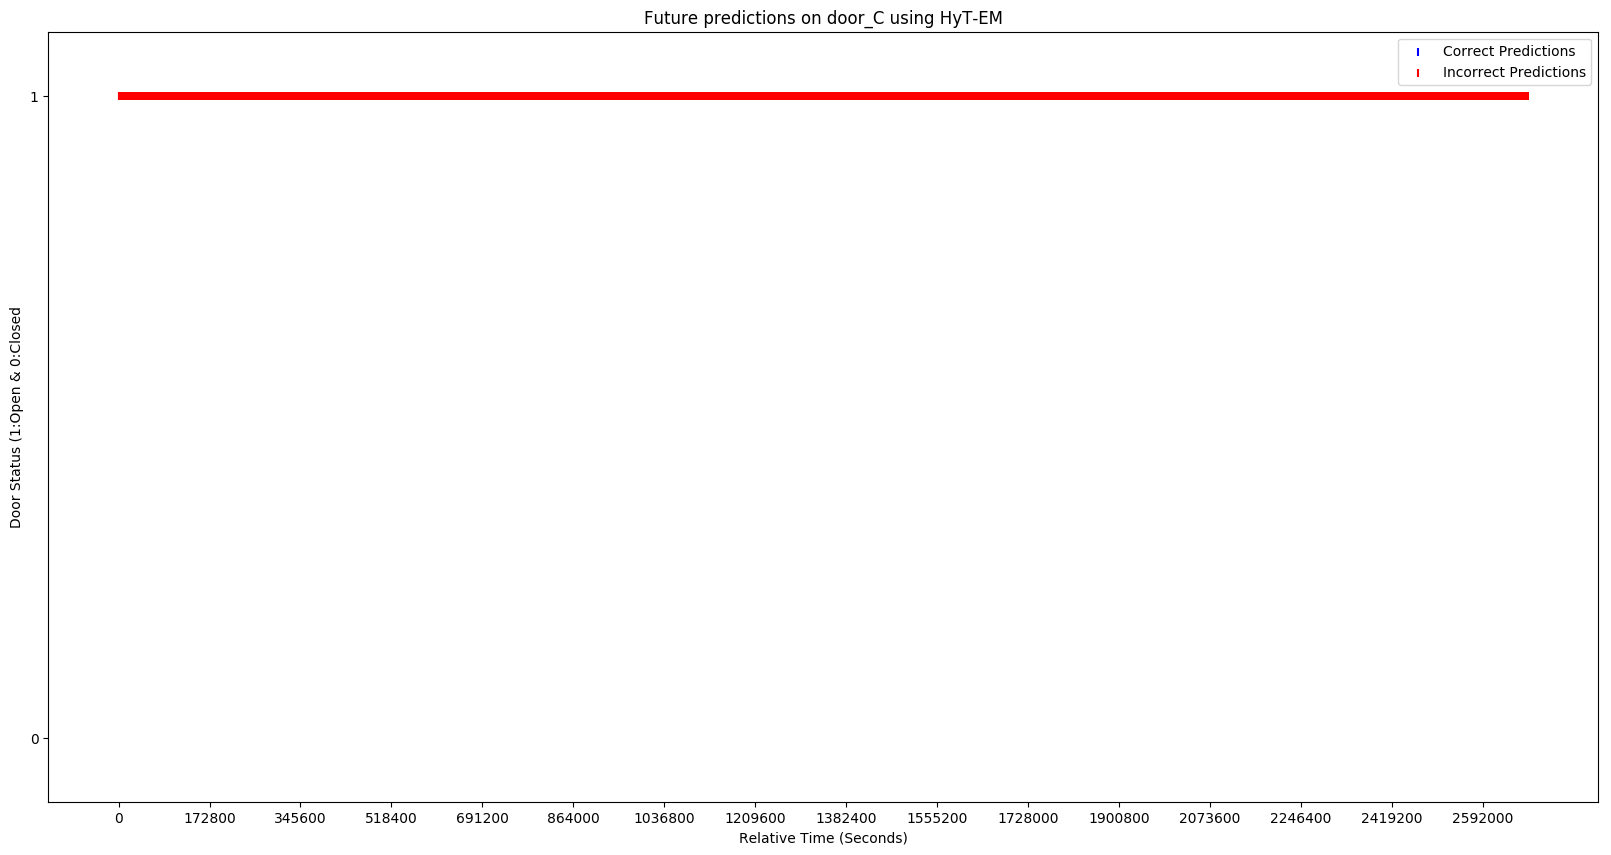
\includegraphics[width = 3in]{images/results/Future_door_C_HyT-EM.png}} \\
  \end{tabular}
  \caption{Future Predictions - Door C}
\end{figure}\\ \\

\begin{figure}
  \begin{tabular}{cc}
    {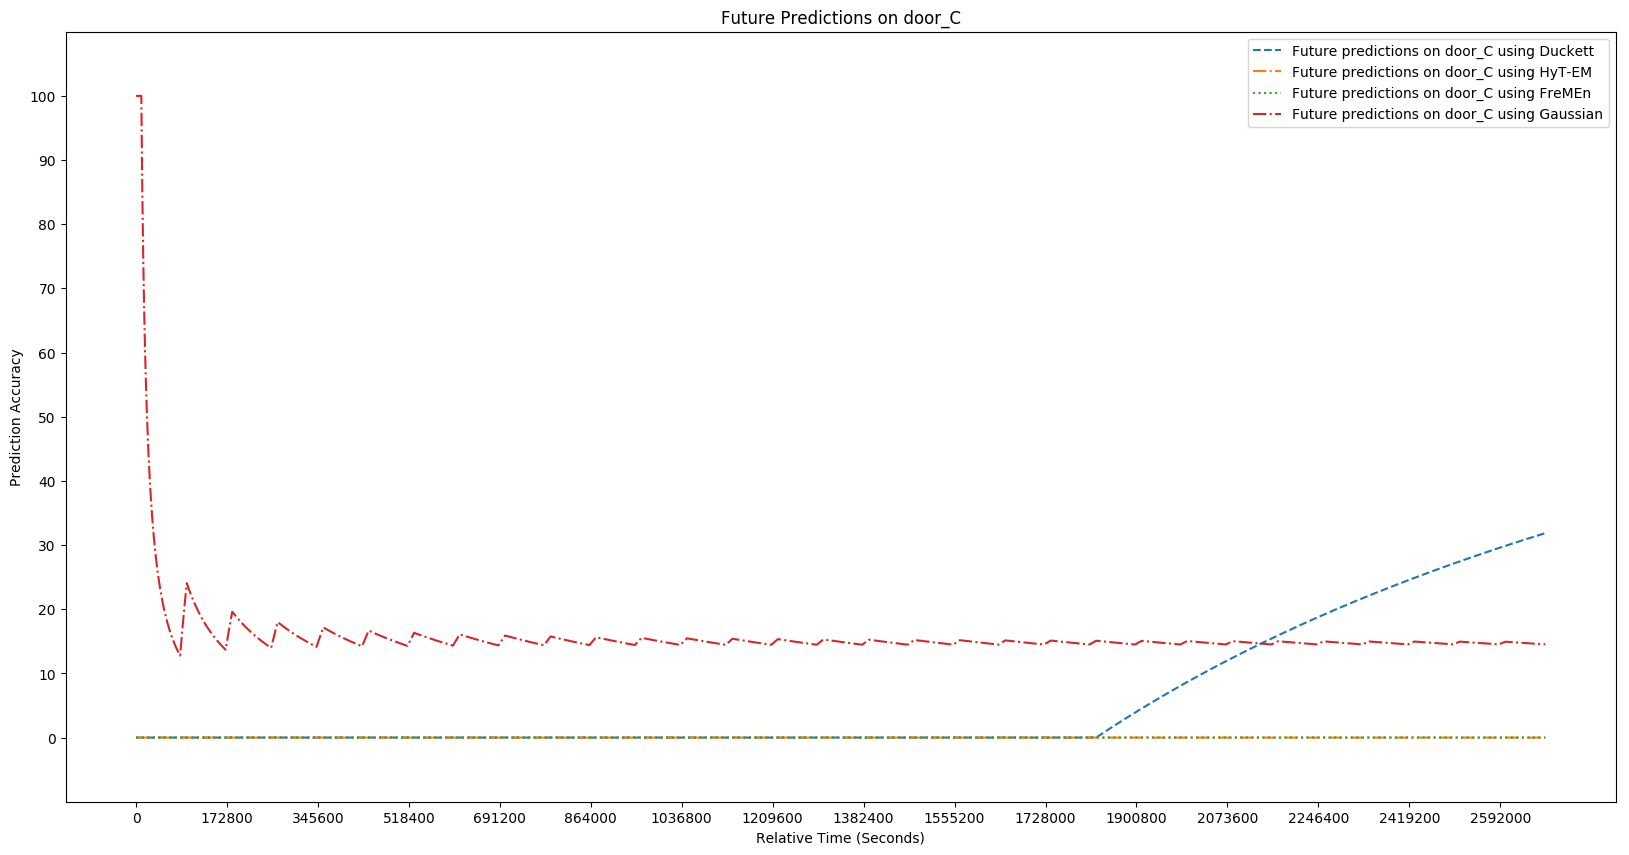
\includegraphics[width = 3in]{images/results/Future_Predictions_on_door_C.png}} &
    {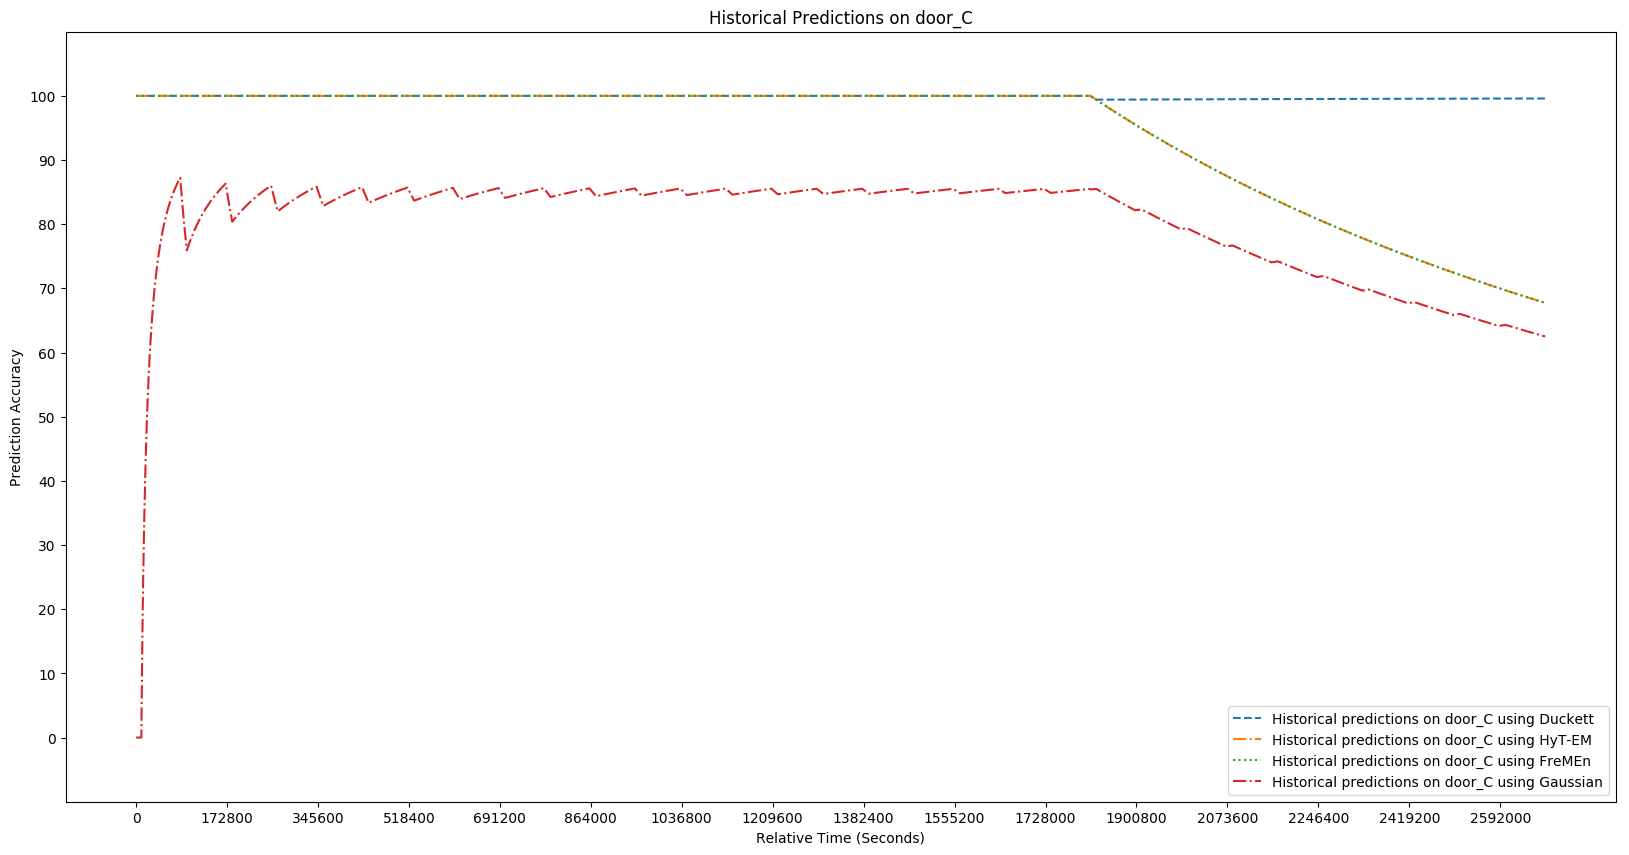
\includegraphics[width = 3in]{images/results/Historical_Predictions_on_door_C.png}} \\
  \end{tabular}
  \caption{Model Accuracy Over Time - Door C}
\end{figure}\\ \\

\subsection{ Final Thoughts }
In terms of memory usage, all four methods appear to be relatively similar, which is to be expected.

\section{ Congested Hallways }
TODO pair down images and move them to the end of the paper


\begin{table}[h!]
  \centering
  \resizebox{\textwidth}{!}{%
    \begin{tabular}{|l|l|l|l|l|}
      \hline
      & Duckett & Gaussian & FreMEn  & HyperTime \\ \hline
      Historical Accuracy             & 91.13\% & 61.49\%  & 64.52\% & 64.52\%   \\ \hline
      Prediction Accuracy             & 32.26\% & 64.05\%  & 63.21\% & 67.74\%   \\ \hline
      Computation Time (Milliseconds) & 600     & 60       & 70      & 1140      \\ \hline
      Memory Usage (KB)               & 31120   & 35364    & 35552   & 37192     \\ \hline
    \end{tabular}%
  }
  \caption{Hallway Trash Section 0}
\end{table}

\begin{table}[h!]
  \centering
  \resizebox{\textwidth}{!}{%
    \begin{tabular}{|l|l|l|l|l|}
      \hline
      & Duckett & Gaussian & FreMEn  & HyperTime \\ \hline
      Historical Accuracy             & 90.96\% & 61.09\%  & 67.74\%  & 67.74\% \\ \hline
      Prediction Accuracy             & 35.79\% & 61.09\%  & 67.74\%  & 67.74\% \\ \hline
      Computation Time (Milliseconds) & 610     & 60       & 70       & 2120    \\ \hline
      Memory Usage (KB)               & 31116   & 35400    & 34928    & 37520   \\ \hline
    \end{tabular}%
  }
  \caption{Hallway Trash Section 1}
\end{table}

\begin{table}[h!]
  \centering
  \resizebox{\textwidth}{!}{%
    \begin{tabular}{|l|l|l|l|l|}
      \hline
      & Duckett & Gaussian & FreMEn  & HyperTime \\ \hline
      Historical Accuracy             & 92.31\% & 55.24\%  & 96.17\% & 99.83\%   \\ \hline
      Prediction Accuracy             & 68.92\% & 55.24\%  & 95.97\% & 99.87\%   \\ \hline
      Computation Time (Milliseconds) & 610     & 60       & 90      & 6790      \\ \hline
      Memory Usage (KB)               & 31032   & 35660    & 35520   & 38372     \\ \hline
    \end{tabular}%
  }
  \caption{Hallway Delivery Section}
\end{table}

\begin{table}[h!]
  \centering
  \resizebox{\textwidth}{!}{%
    \begin{tabular}{|l|l|l|l|l|}
      \hline
      & Duckett & Gaussian & FreMEn  & HyperTime \\ \hline
      Historical Accuracy             & 61.63\% & 52.08\%  & 100.00\% & 100.00\% \\ \hline
      Prediction Accuracy             & 61.63\% & 52.08\%  & 100.00\% & 100.00\% \\ \hline
      Computation Time (Milliseconds) & 620     & 60       & 70       & 880      \\ \hline
      Memory Usage (KB)               & 30896   & 35524    & 35600    & 38288    \\ \hline
    \end{tabular}%
  }
  \caption{Hallway Meal Section 0}
\end{table}

\begin{table}[h!]
  \centering
  \resizebox{\textwidth}{!}{%
    \begin{tabular}{|l|l|l|l|l|}
      \hline
      & Duckett & Gaussian & FreMEn  & HyperTime \\ \hline
      Historical Accuracy             & 74.93\% & 65.62\%  & 100.00\% & 100.00\% \\ \hline
      Prediction Accuracy             & 74.93\% & 65.62\%  & 100.00\% & 100.00\% \\ \hline
      Computation Time (Milliseconds) & 600     & 60       & 70       & 990      \\ \hline
      Memory Usage (KB)               & 31384   & 35388    & 35588    & 37608    \\ \hline
    \end{tabular}%
  }
  \caption{Hallway Meal Section 1}
\end{table}

\begin{table}[h!]
  \centering
  \resizebox{\textwidth}{!}{%
    \begin{tabular}{|l|l|l|l|l|}
      \hline
      & Duckett & Gaussian & FreMEn  & HyperTime \\ \hline
      Historical Accuracy             & 78.93\% & 26.04\%  & 100.00\% & 100.00\% \\ \hline
      Prediction Accuracy             & 78.93\% & 26.04\%  & 100.00\% & 100.00\% \\ \hline
      Computation Time (Milliseconds) & 610     & 60       & 70       & 1860     \\ \hline
      Memory Usage (KB)               & 30984   & 35160    & 35172    & 37632    \\ \hline
    \end{tabular}%
  }
  \caption{Hallway Laundry Section}
\end{table}

\begin{table}[h!]
  \centering
  \resizebox{\textwidth}{!}{%
    \begin{tabular}{|l|l|l|l|l|}
      \hline
      & Duckett & Gaussian & FreMEn  & HyperTime \\ \hline
      Number of Hard Errors              & 1790   & 2418   & 1488   & 1488 \\ \hline
      Number of Soft Errors              & 442    & 62     & 80     & 80   \\ \hline
      Average Additional Cells Traversed & 5.74   & 6.34   & 3.12   & 3.12 \\ \hline
    \end{tabular}%
  }
  \caption{Historical Path Planning Results}
\end{table}

\begin{table}[h!]
  \centering
  \resizebox{\textwidth}{!}{%
    \begin{tabular}{|l|l|l|l|l|}
      \hline
      & Duckett & Gaussian & FreMEn  & HyperTime \\ \hline
      Number of Hard Errors              & 1790   & 2418   & 1488   & 1488 \\ \hline
      Number of Soft Errors              & 444    & 62     & 80     & 80   \\ \hline
      Average Additional Cells Traversed & 5.74   & 6.34   & 3.12   & 3.12 \\ \hline
    \end{tabular}%
  }
  \caption{Future Path Planning Results}
\end{table} \\ \\ \\









\begin{figure}
  \begin{tabular}{cc}
    {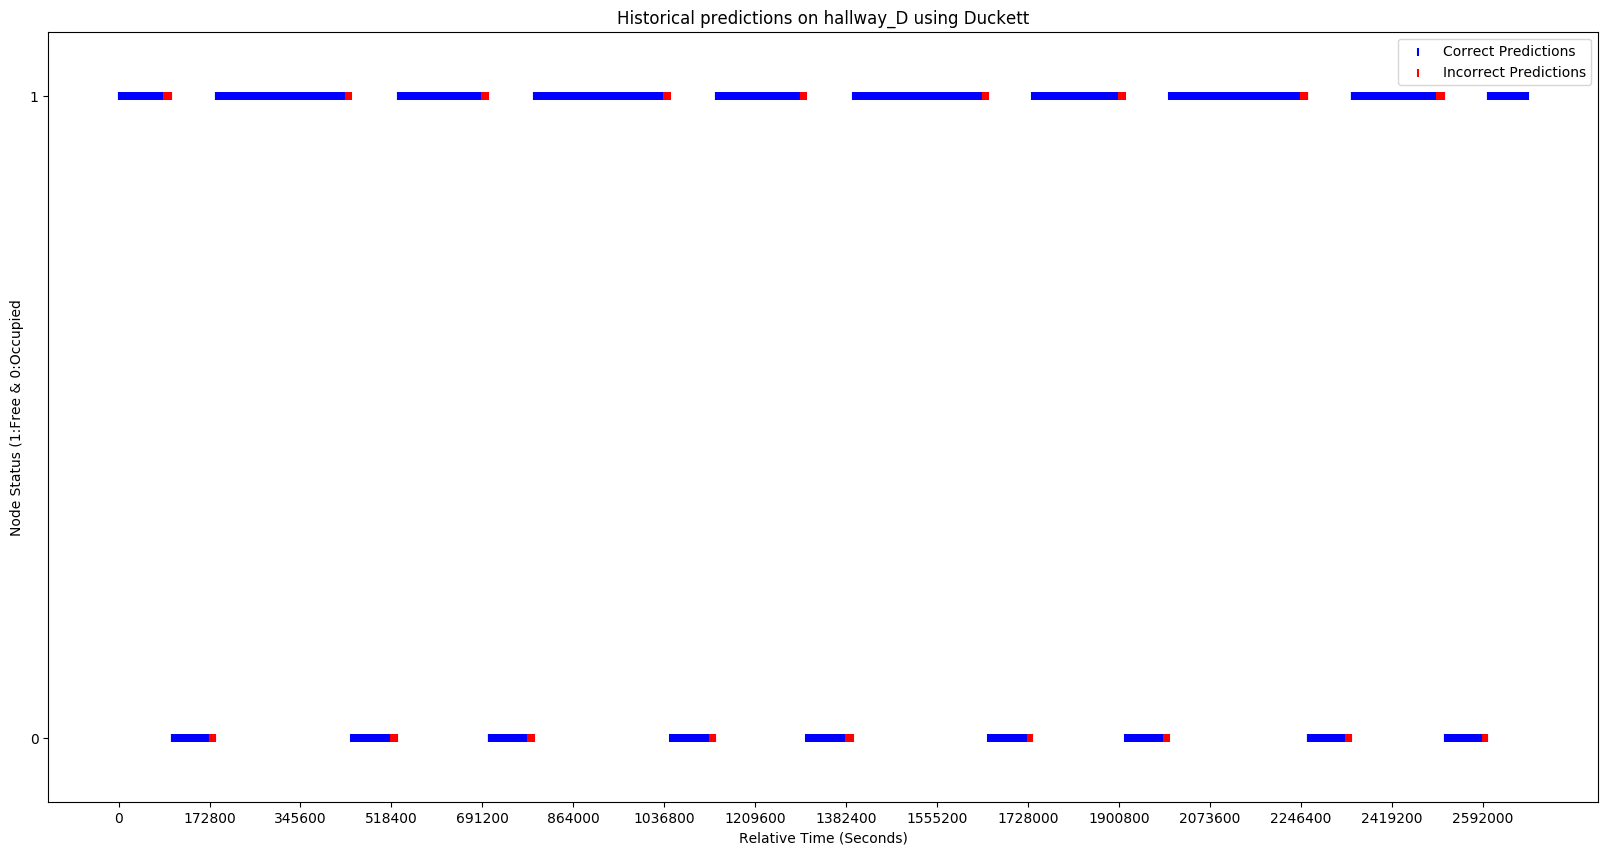
\includegraphics[width = 3in]{images/results/Historical_hallway_D_Duckett.png}} &
    {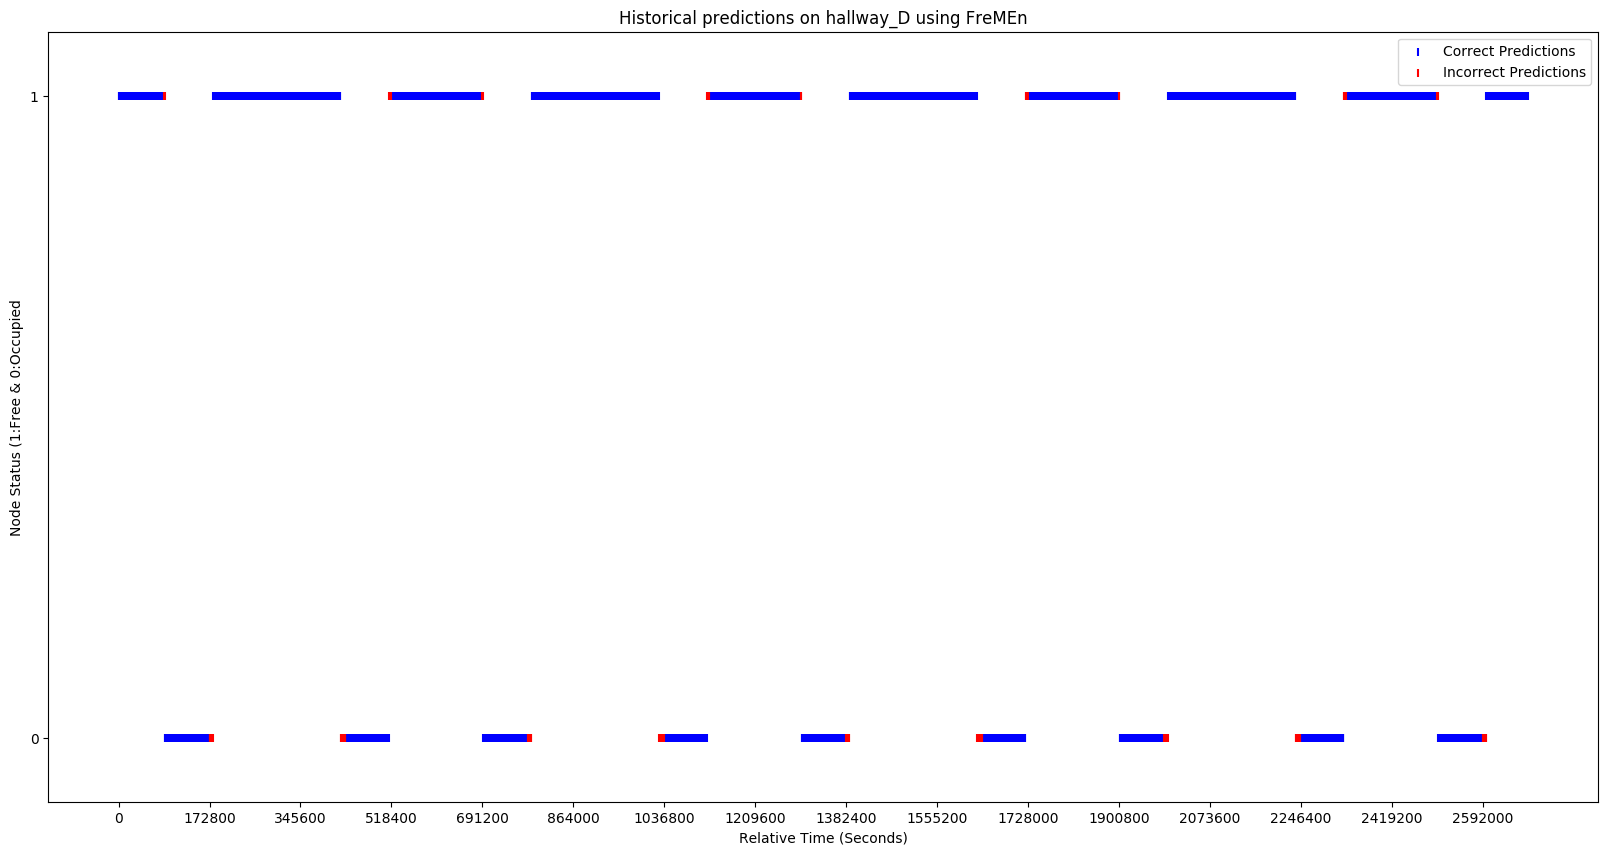
\includegraphics[width = 3in]{images/results/Historical_hallway_D_FreMEn.png}} \\
    {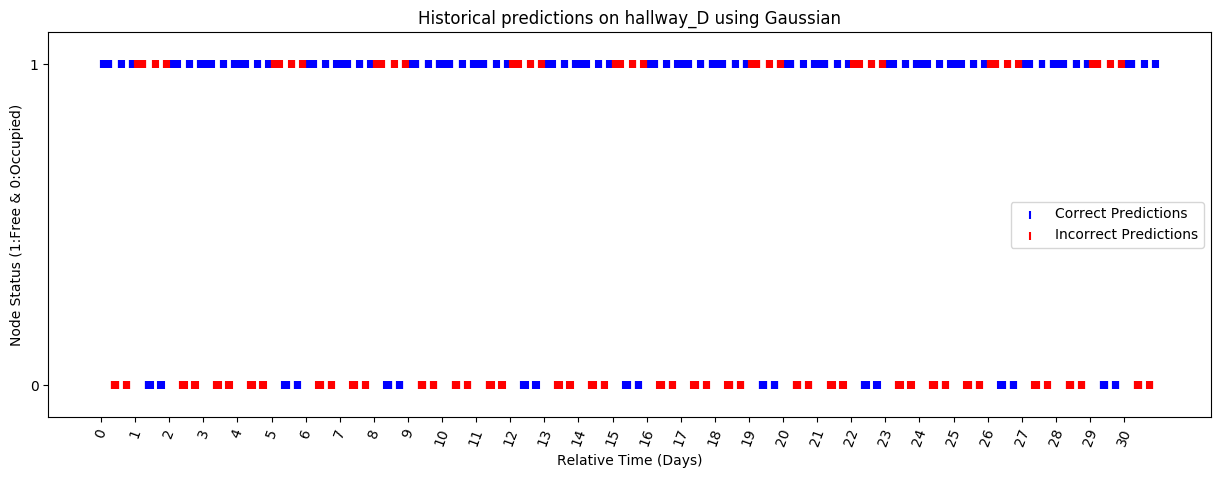
\includegraphics[width = 3in]{images/results/Historical_hallway_D_Gaussian.png}} &
    {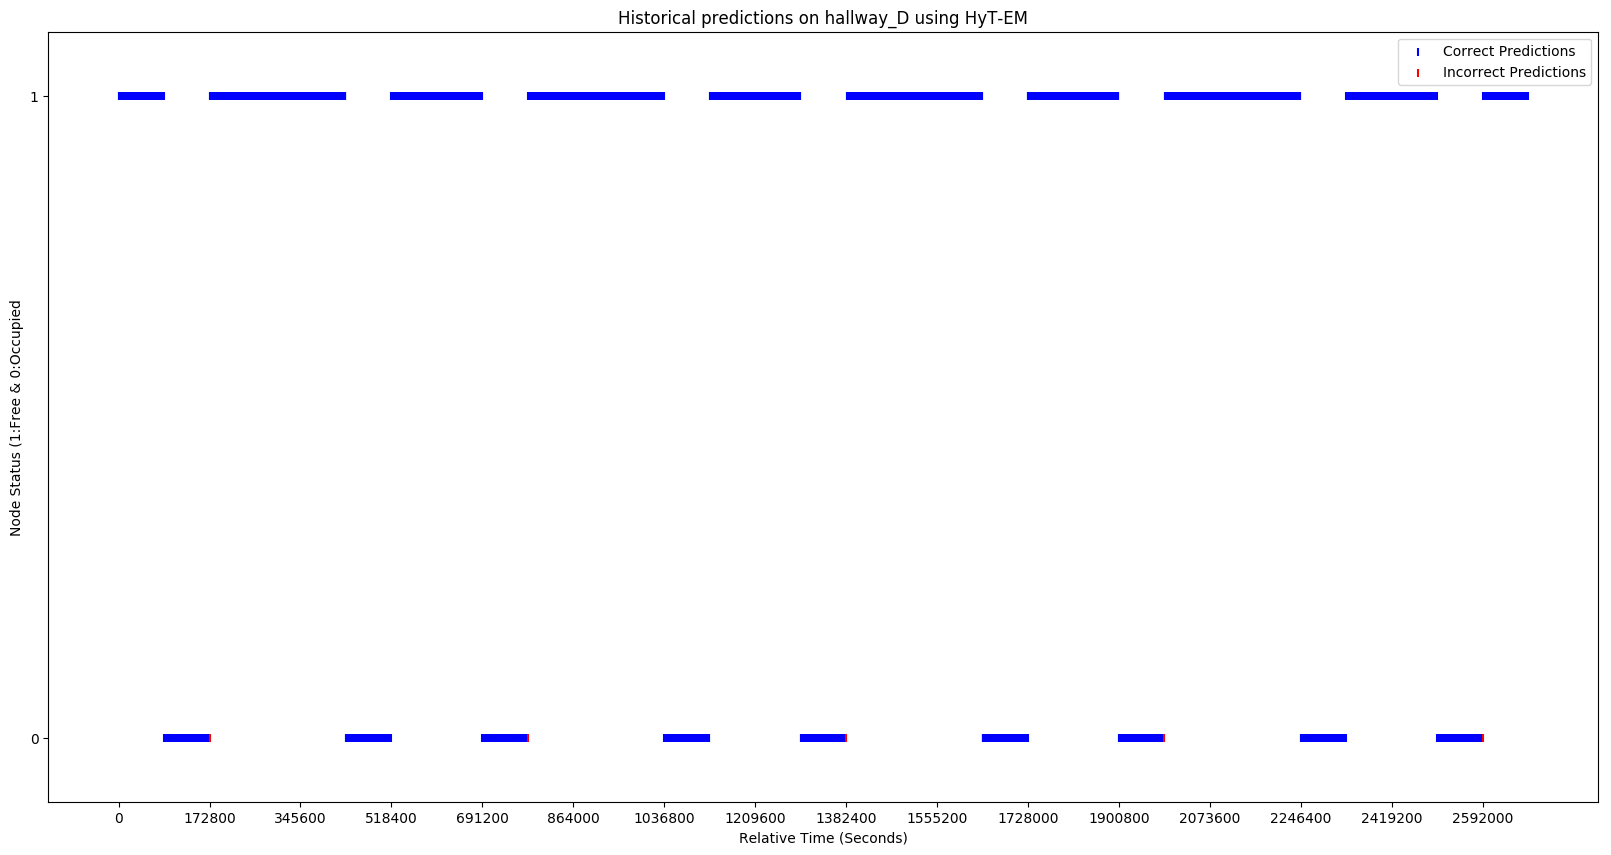
\includegraphics[width = 3in]{images/results/Historical_hallway_D_HyT-EM.png}} \\
  \end{tabular}
  \caption{Historical Recreations - Hallway Delivery}
\end{figure}\\ \\

\begin{figure}
  \begin{tabular}{cc}
    {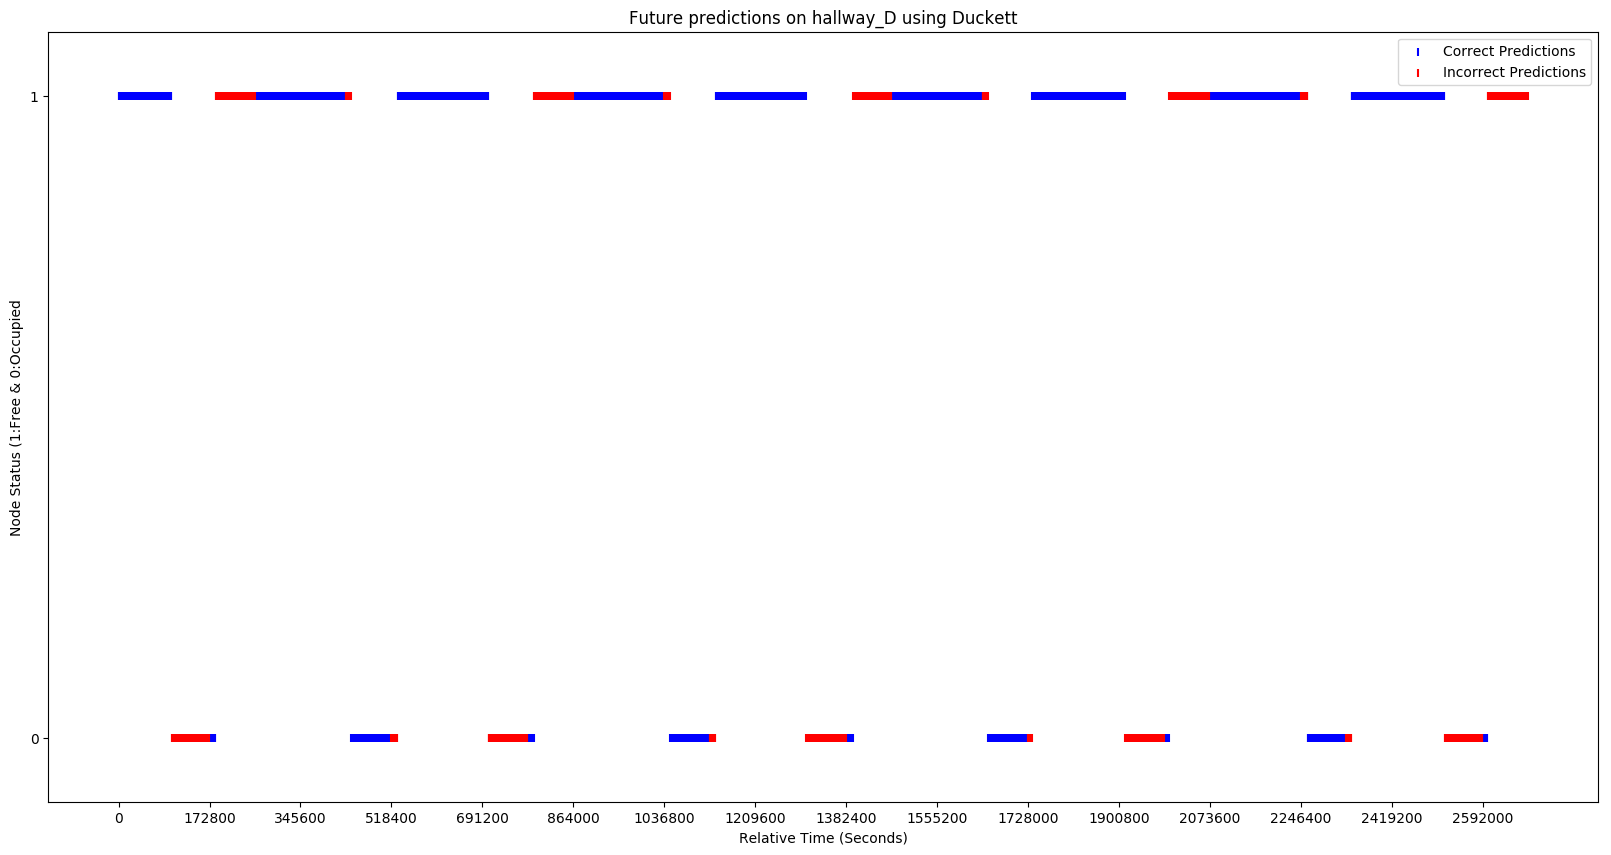
\includegraphics[width = 3in]{images/results/Future_hallway_D_Duckett.png}} &
    {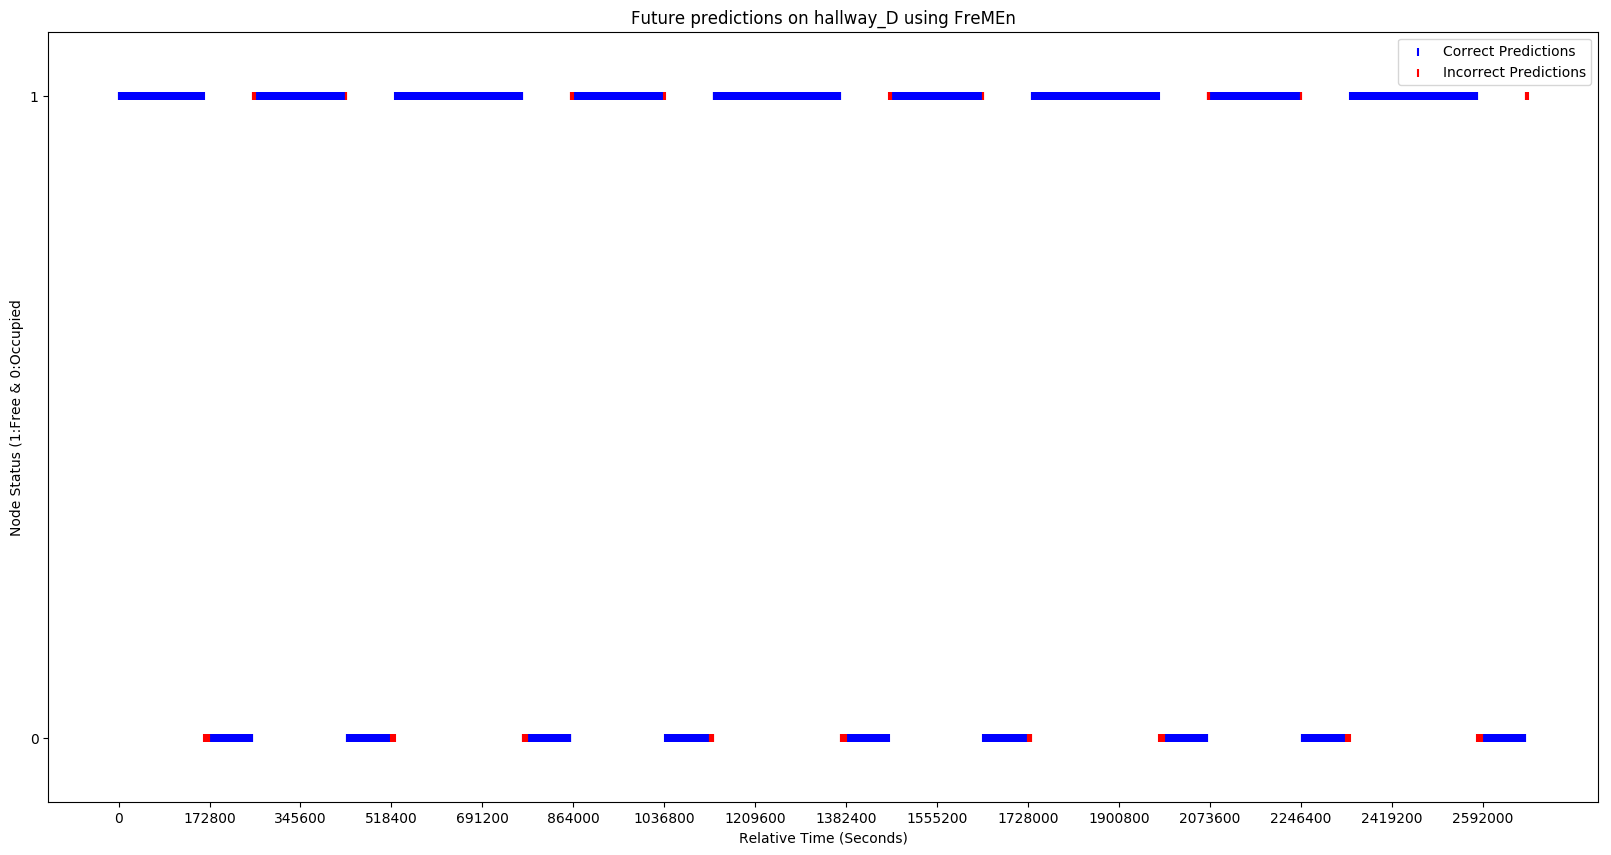
\includegraphics[width = 3in]{images/results/Future_hallway_D_FreMEn.png}} \\
    {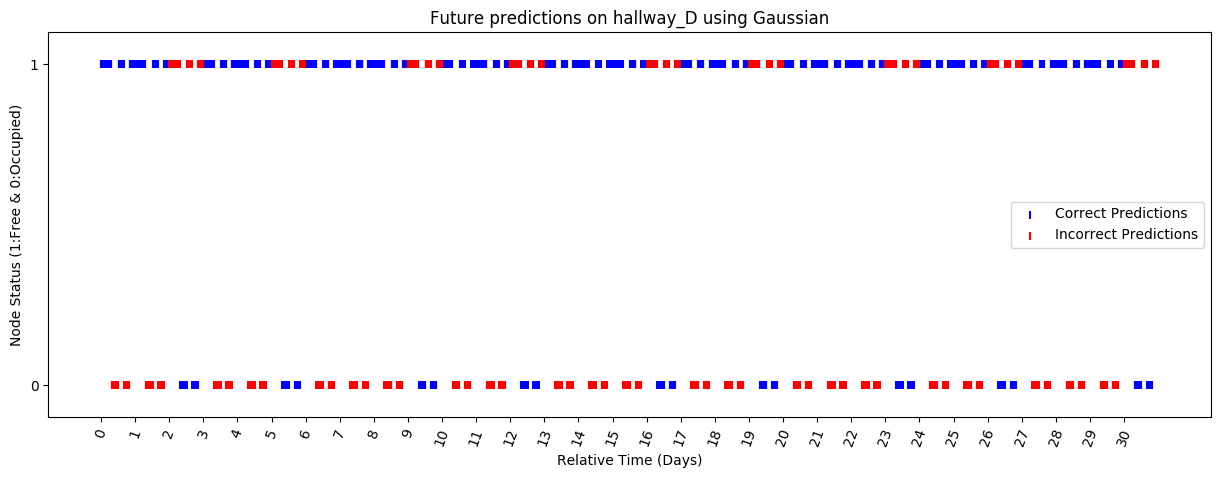
\includegraphics[width = 3in]{images/results/Future_hallway_D_Gaussian.png}} &
    {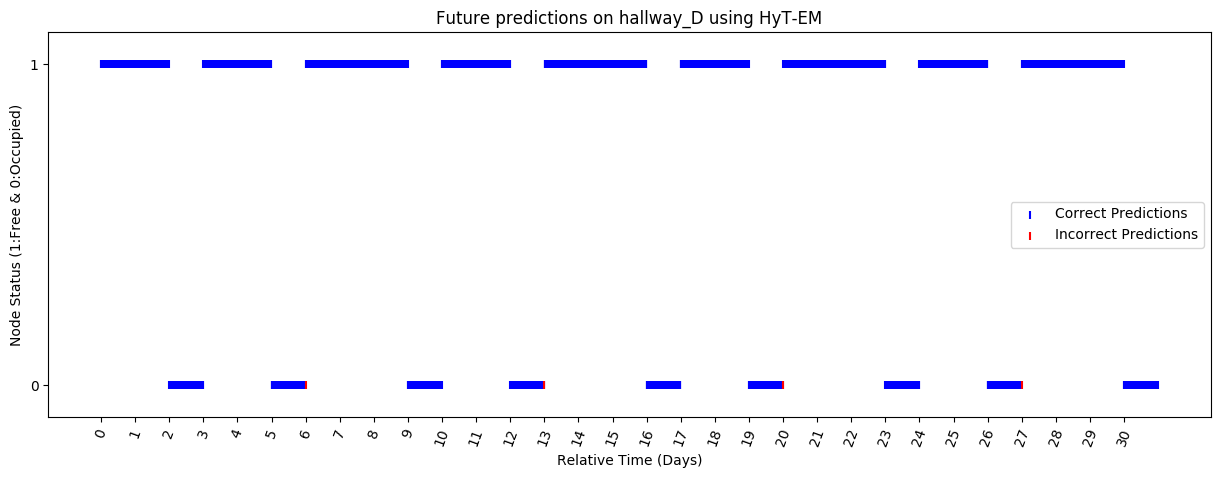
\includegraphics[width = 3in]{images/results/Future_hallway_D_HyT-EM.png}} \\
  \end{tabular}
  \caption{Future Predictions - Hallway Delivery}
\end{figure}\\ \\

\begin{figure}
  \begin{tabular}{cc}
    {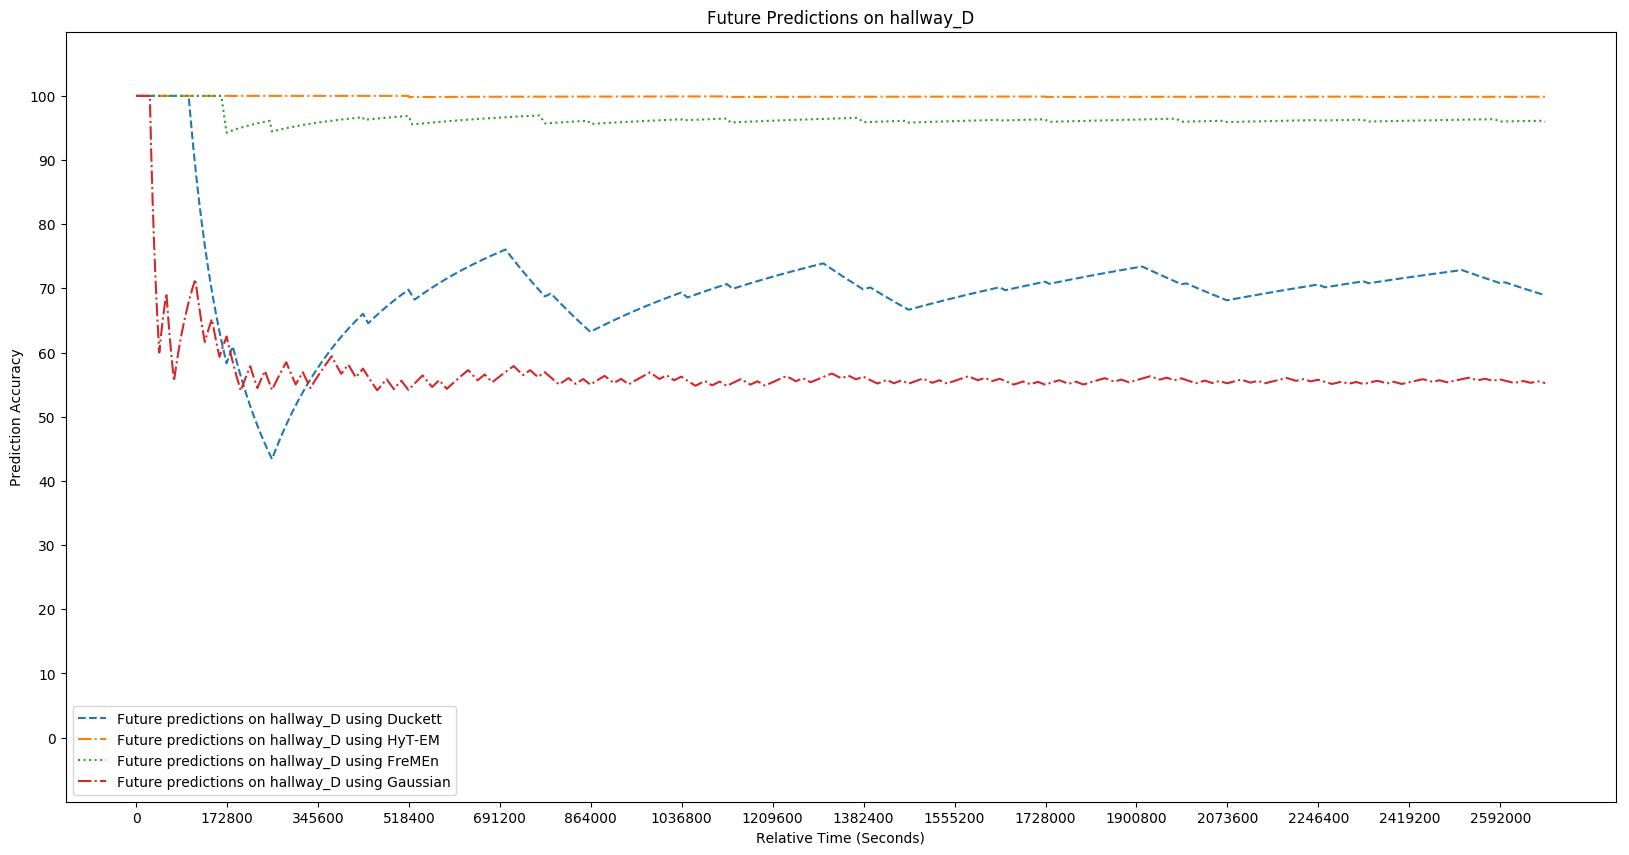
\includegraphics[width = 3in]{images/results/Future_Predictions_on_hallway_D.png}} &
    {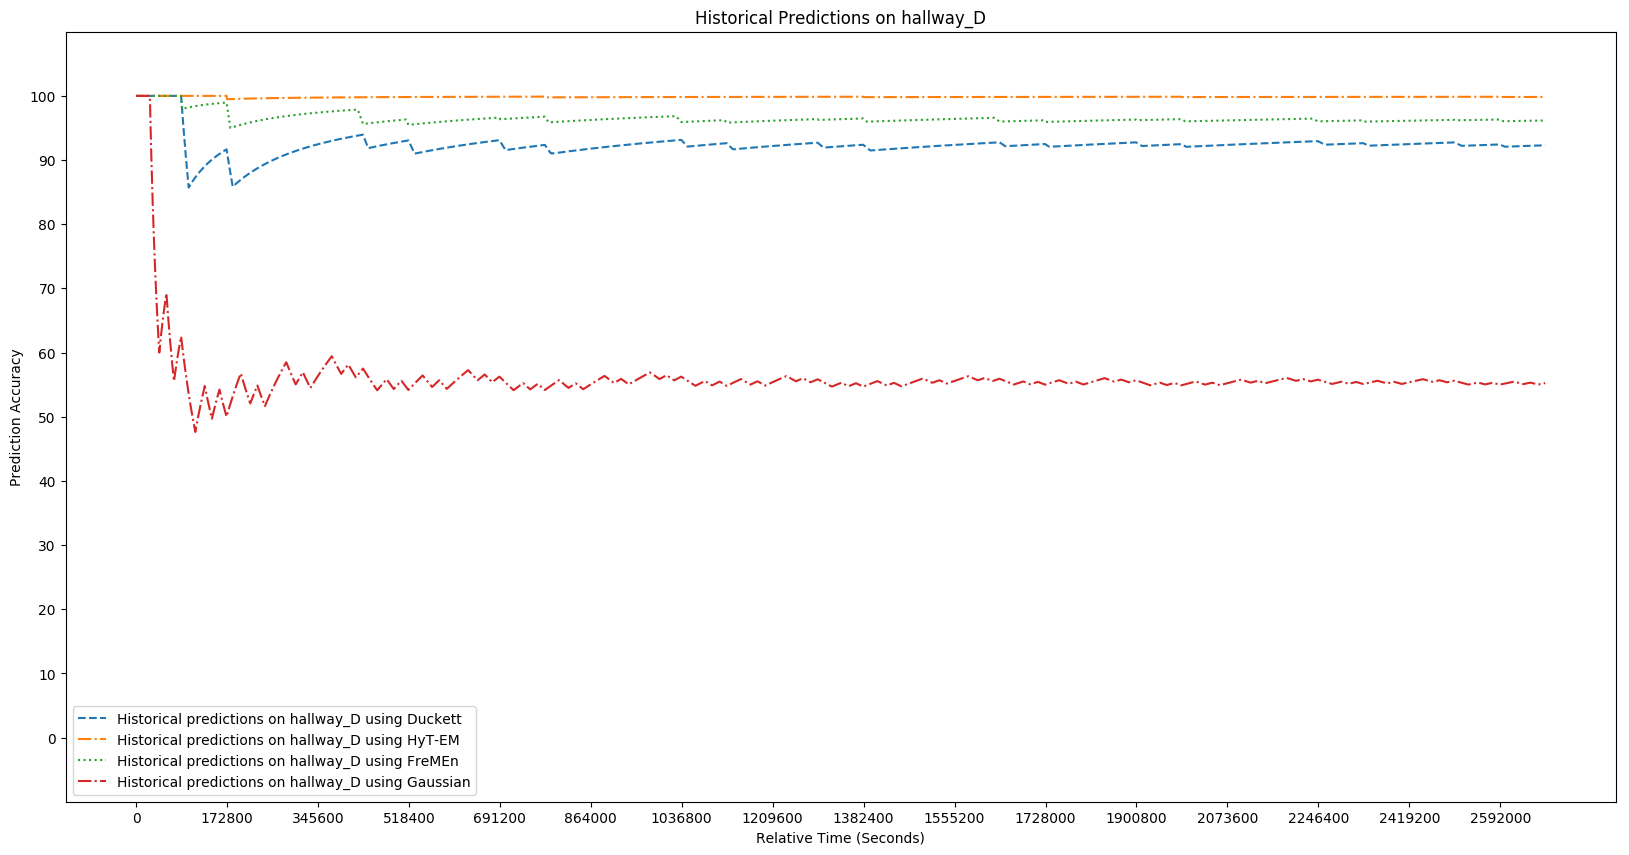
\includegraphics[width = 3in]{images/results/Historical_Predictions_on_hallway_D.png}} \\
  \end{tabular}
  \caption{Model Accuracy Over Time - Hallway Delivery}
\end{figure}\\ \\


\begin{figure}
  \begin{tabular}{cc}
    {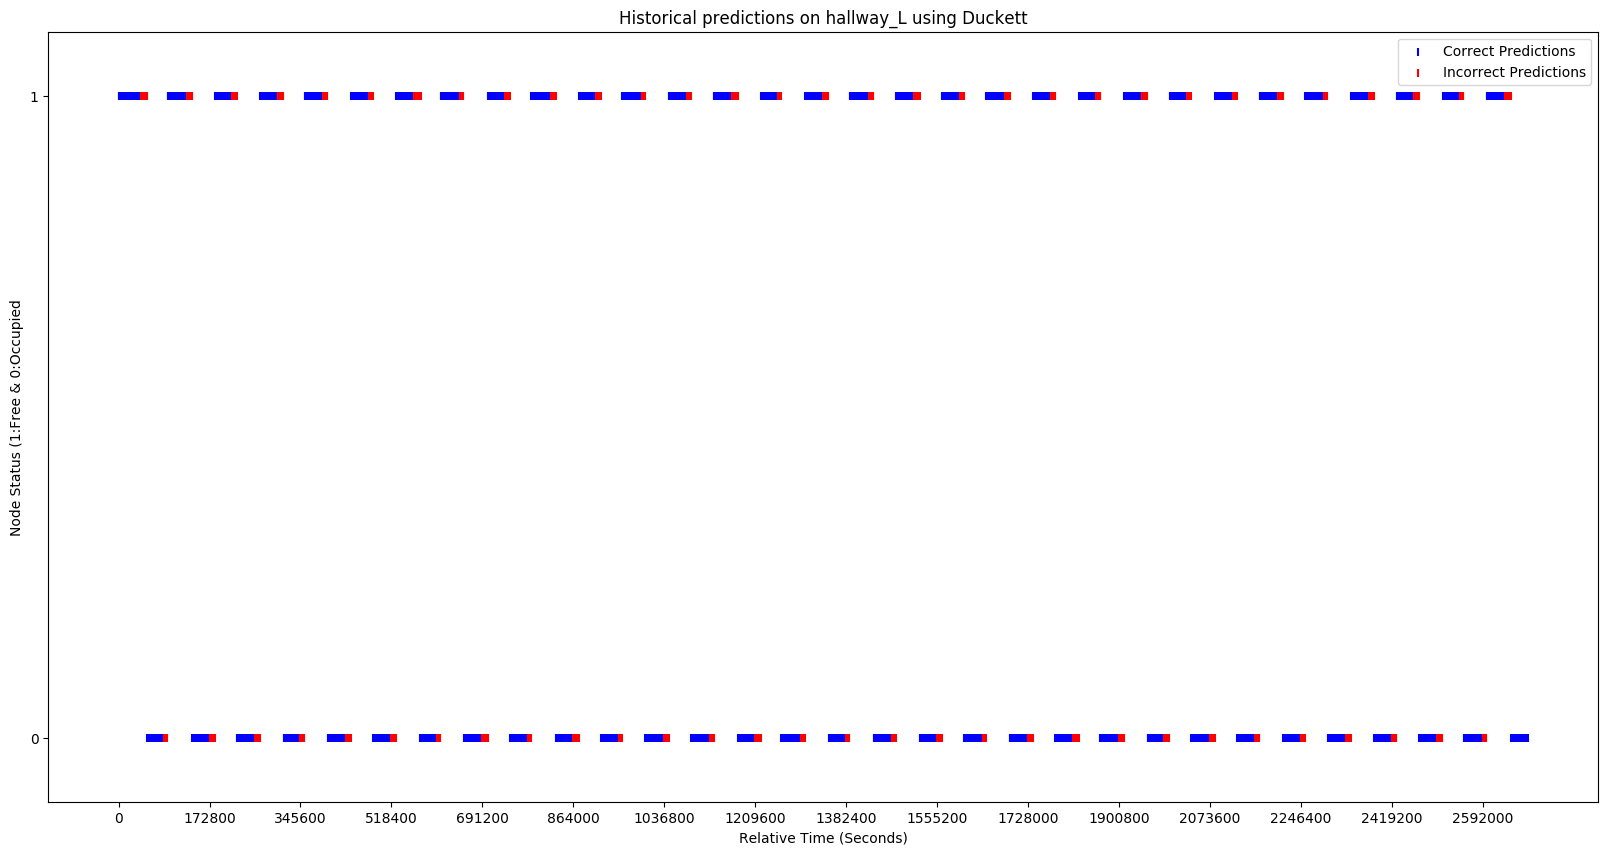
\includegraphics[width = 3in]{images/results/Historical_hallway_L_Duckett.png}} &
    {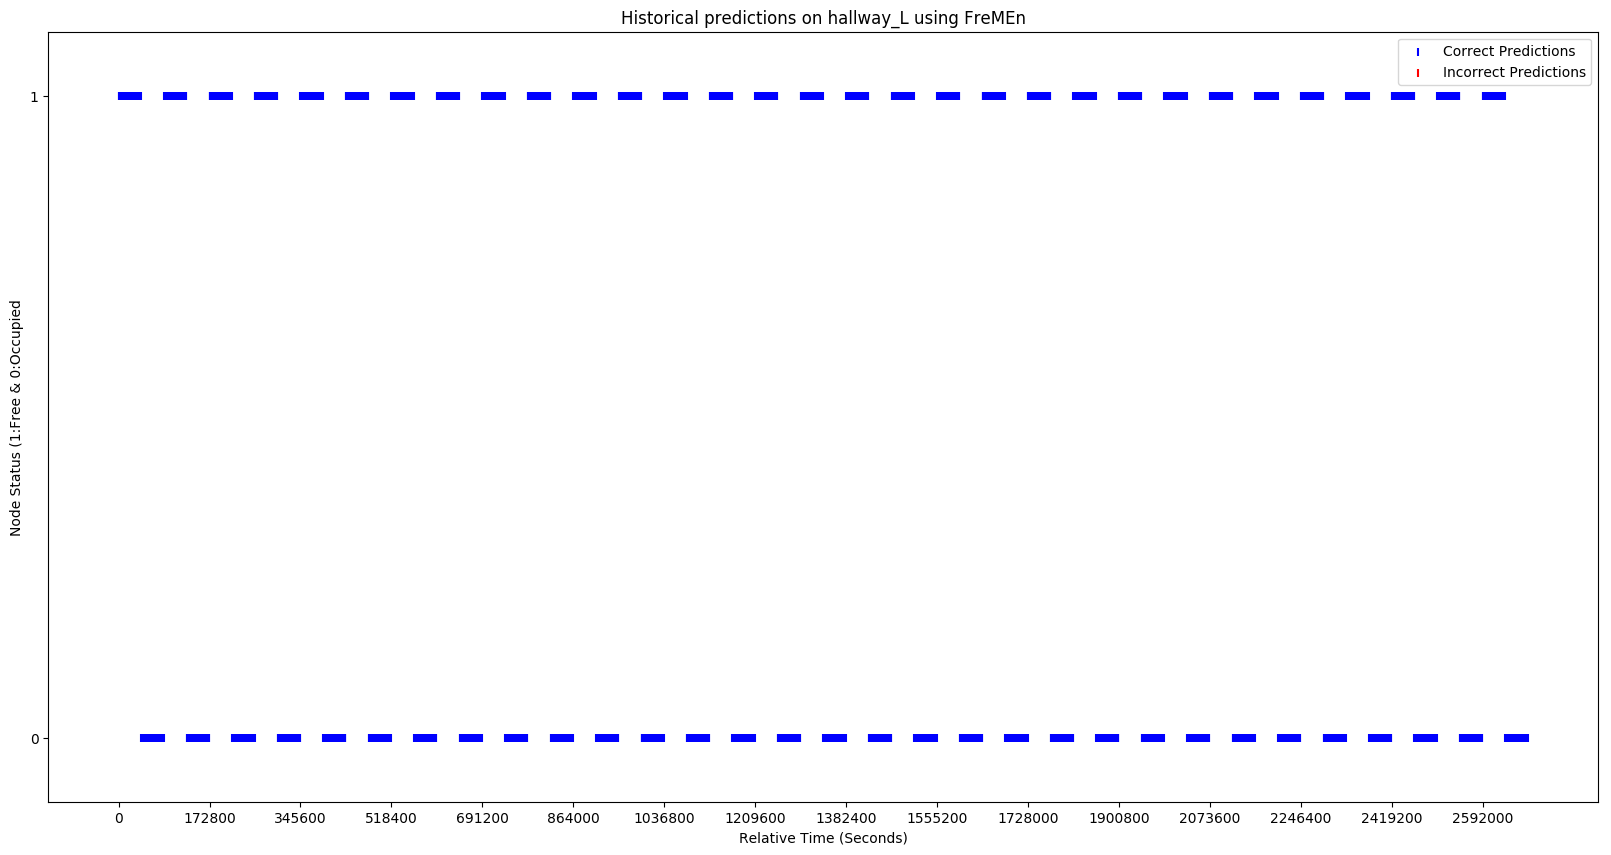
\includegraphics[width = 3in]{images/results/Historical_hallway_L_FreMEn.png}} \\
    {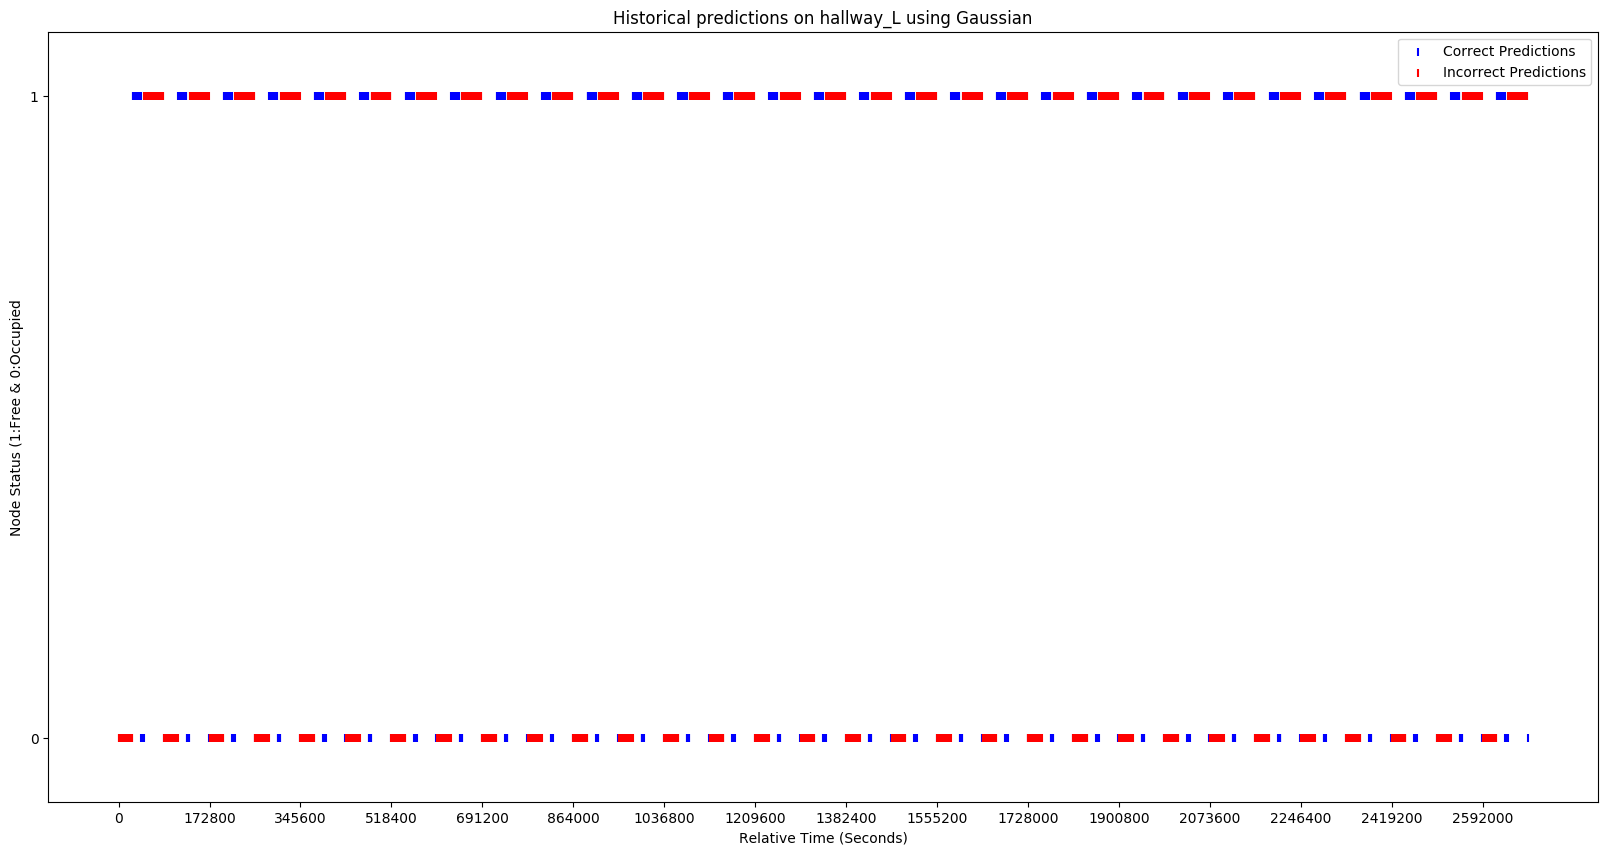
\includegraphics[width = 3in]{images/results/Historical_hallway_L_Gaussian.png}} &
    {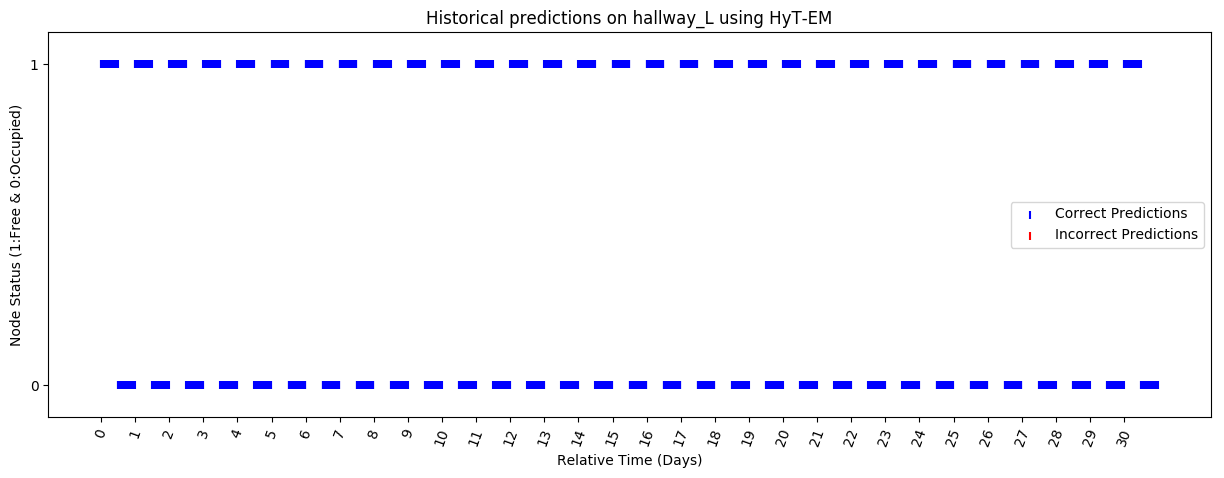
\includegraphics[width = 3in]{images/results/Historical_hallway_L_HyT-EM.png}} \\
  \end{tabular}
  \caption{Historical Recreations - Hallway Delivery}
\end{figure}\\ \\

\begin{figure}
  \begin{tabular}{cc}
    {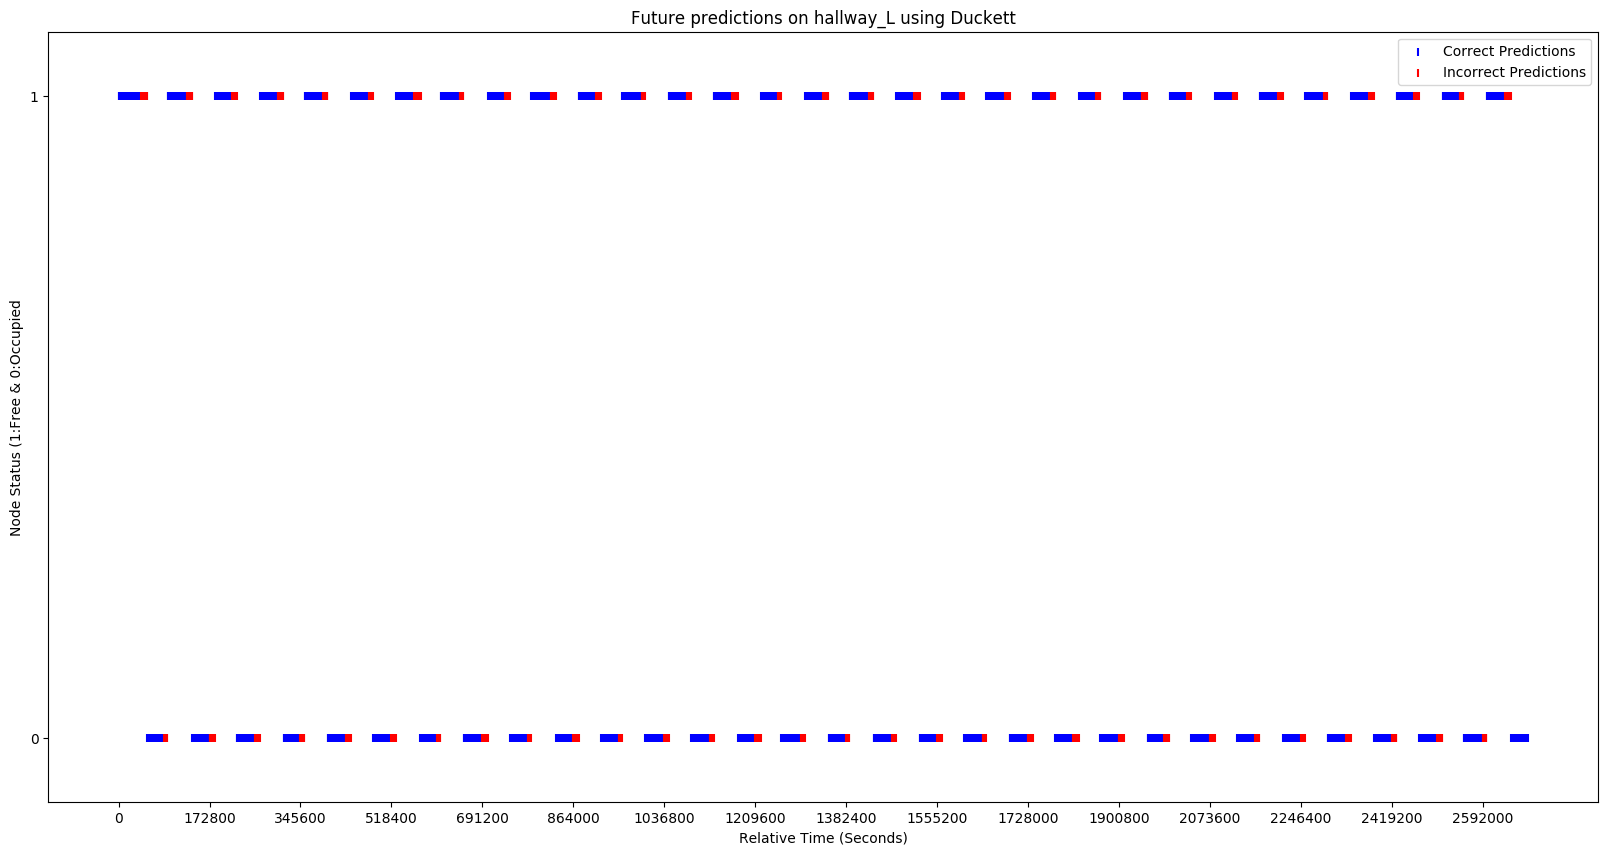
\includegraphics[width = 3in]{images/results/Future_hallway_L_Duckett.png}} &
    {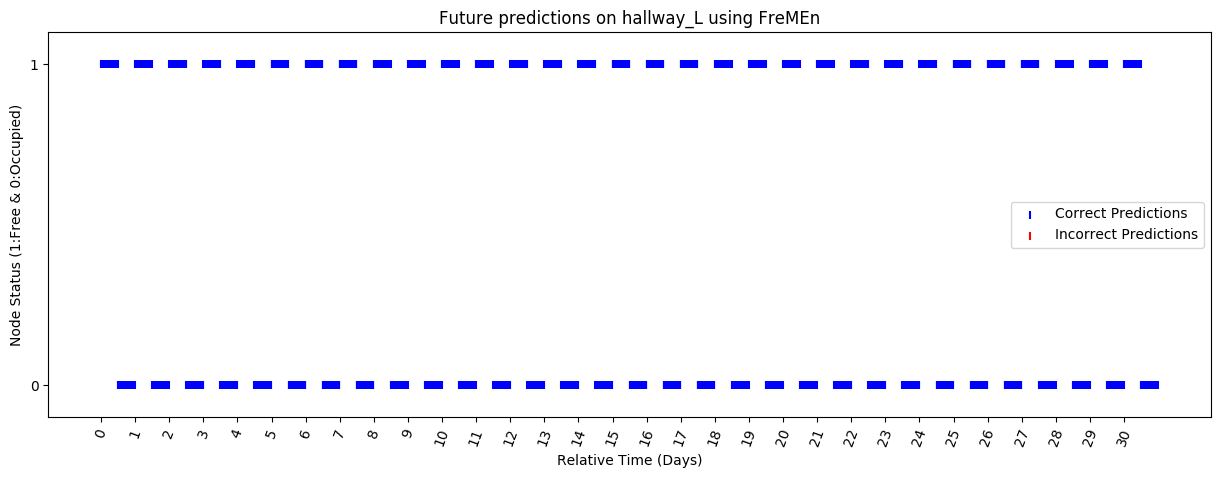
\includegraphics[width = 3in]{images/results/Future_hallway_L_FreMEn.png}} \\
    {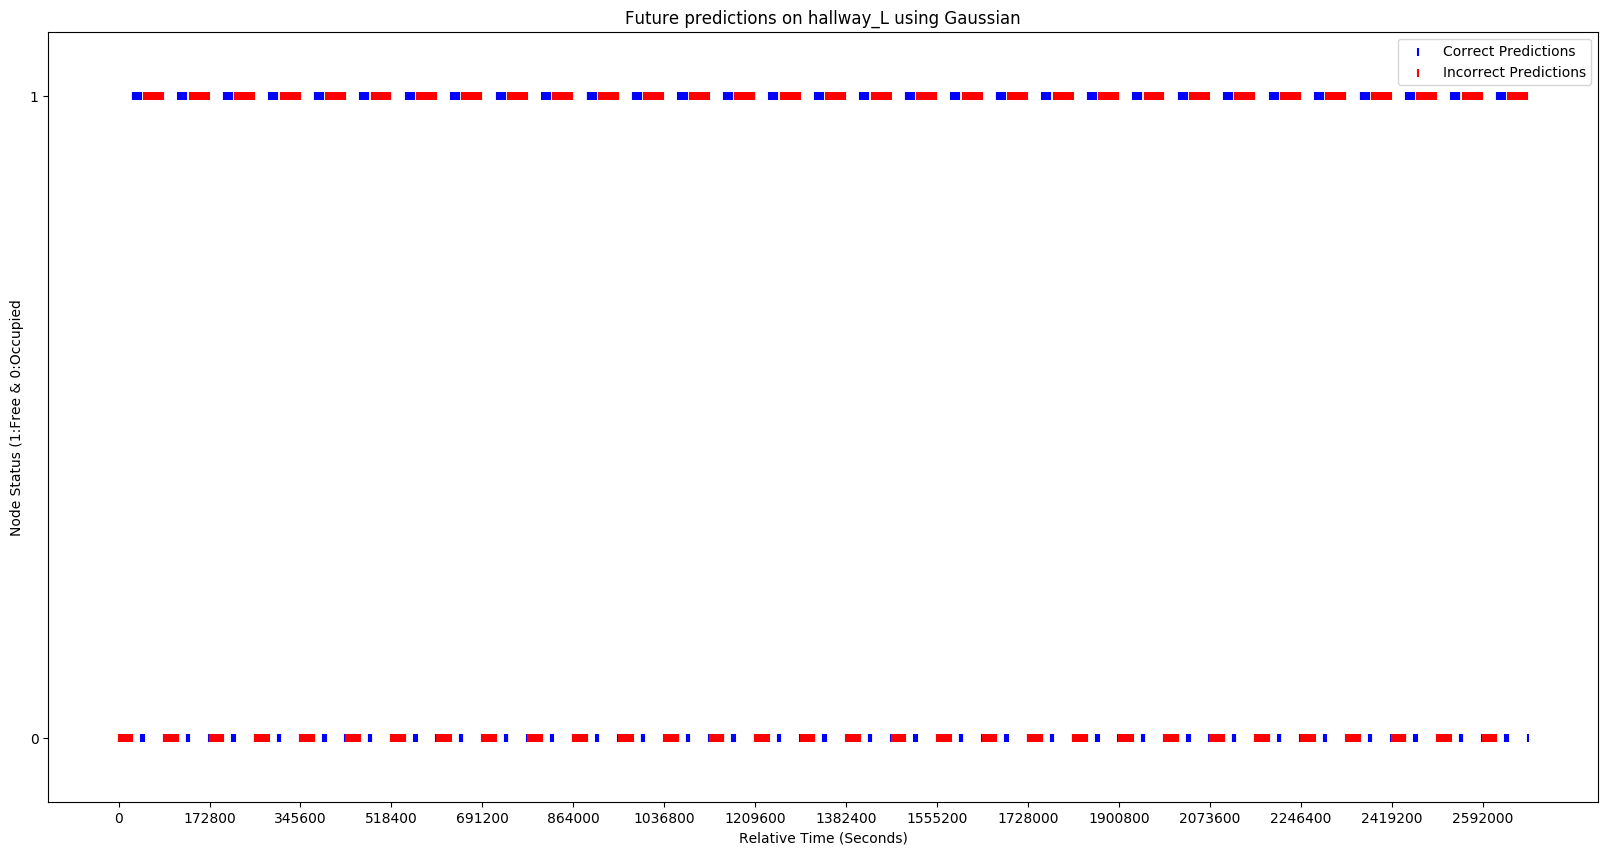
\includegraphics[width = 3in]{images/results/Future_hallway_L_Gaussian.png}} &
    {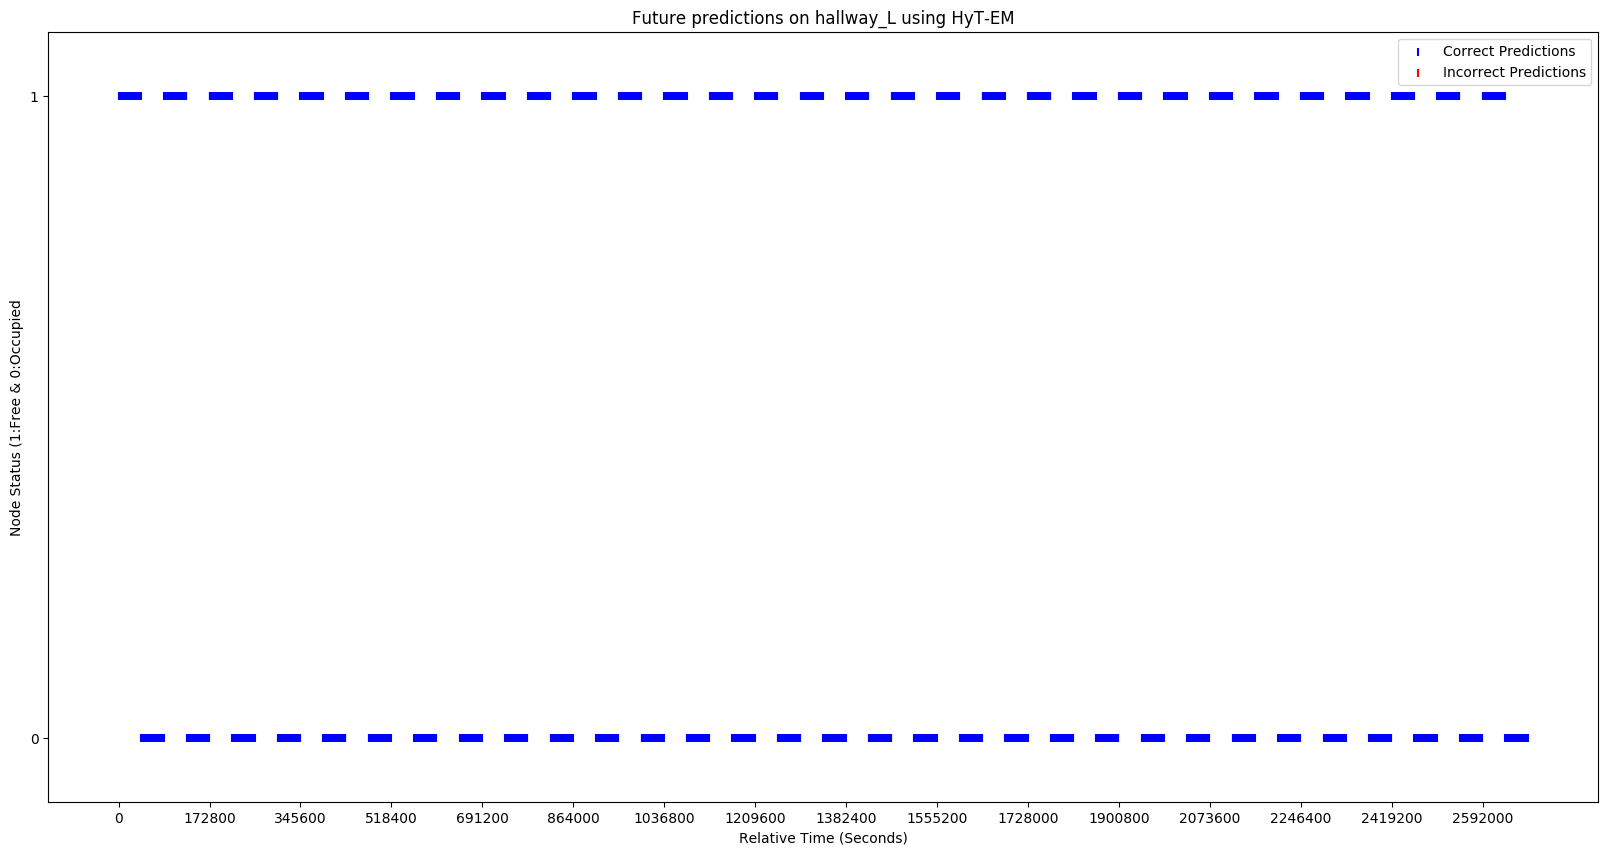
\includegraphics[width = 3in]{images/results/Future_hallway_L_HyT-EM.png}} \\
  \end{tabular}
  \caption{Future Predictions - Hallway Laundry}
\end{figure}\\ \\

\begin{figure}
  \begin{tabular}{cc}
    {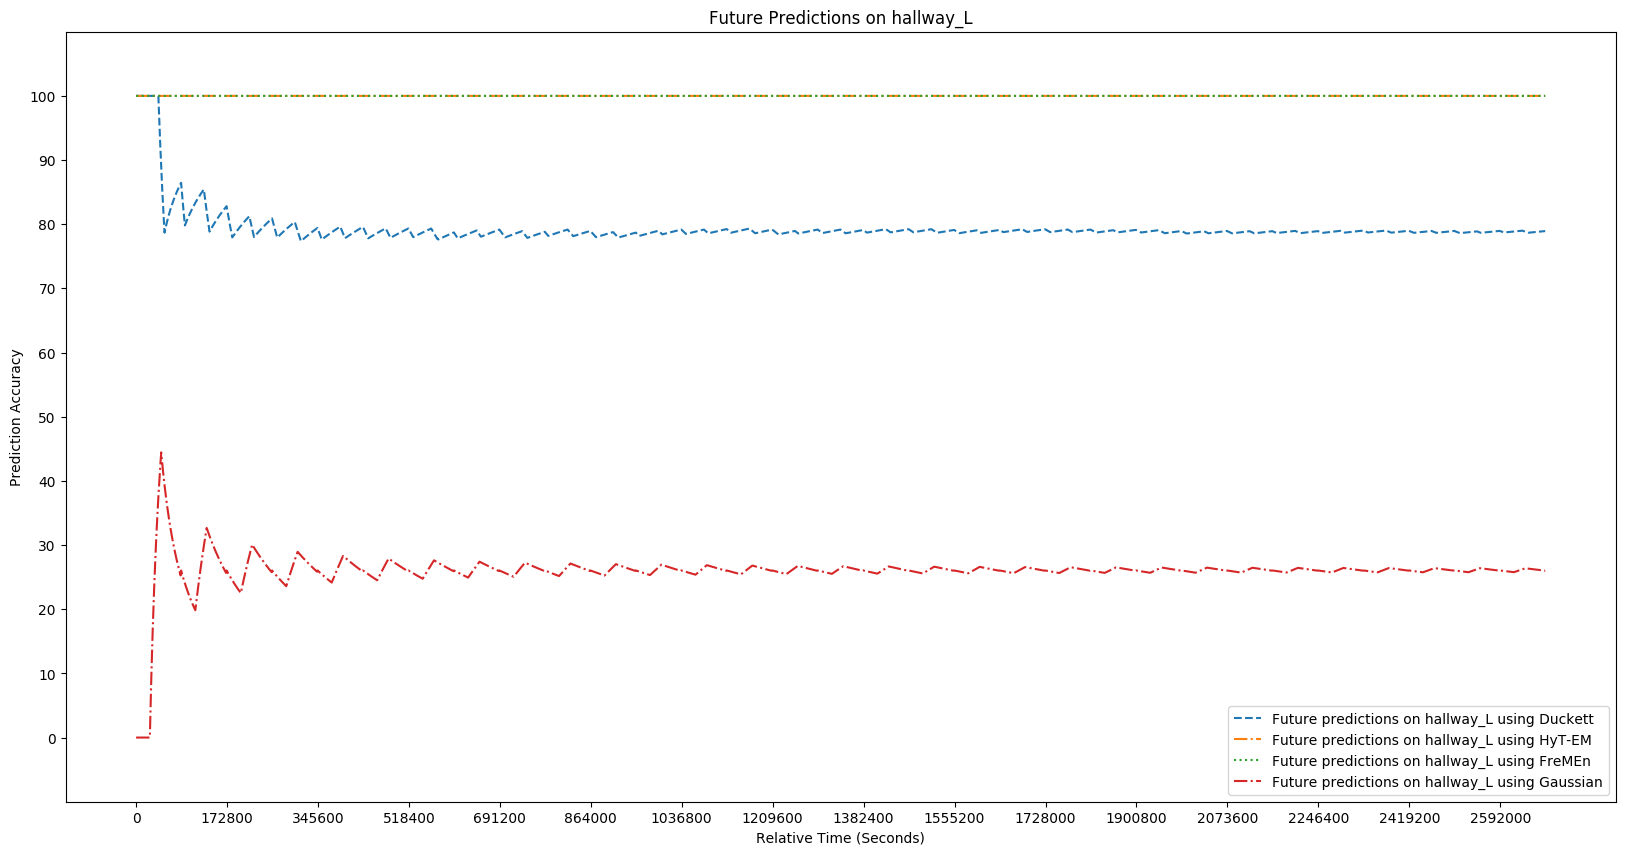
\includegraphics[width = 3in]{images/results/Future_Predictions_on_hallway_L.png}} &
    {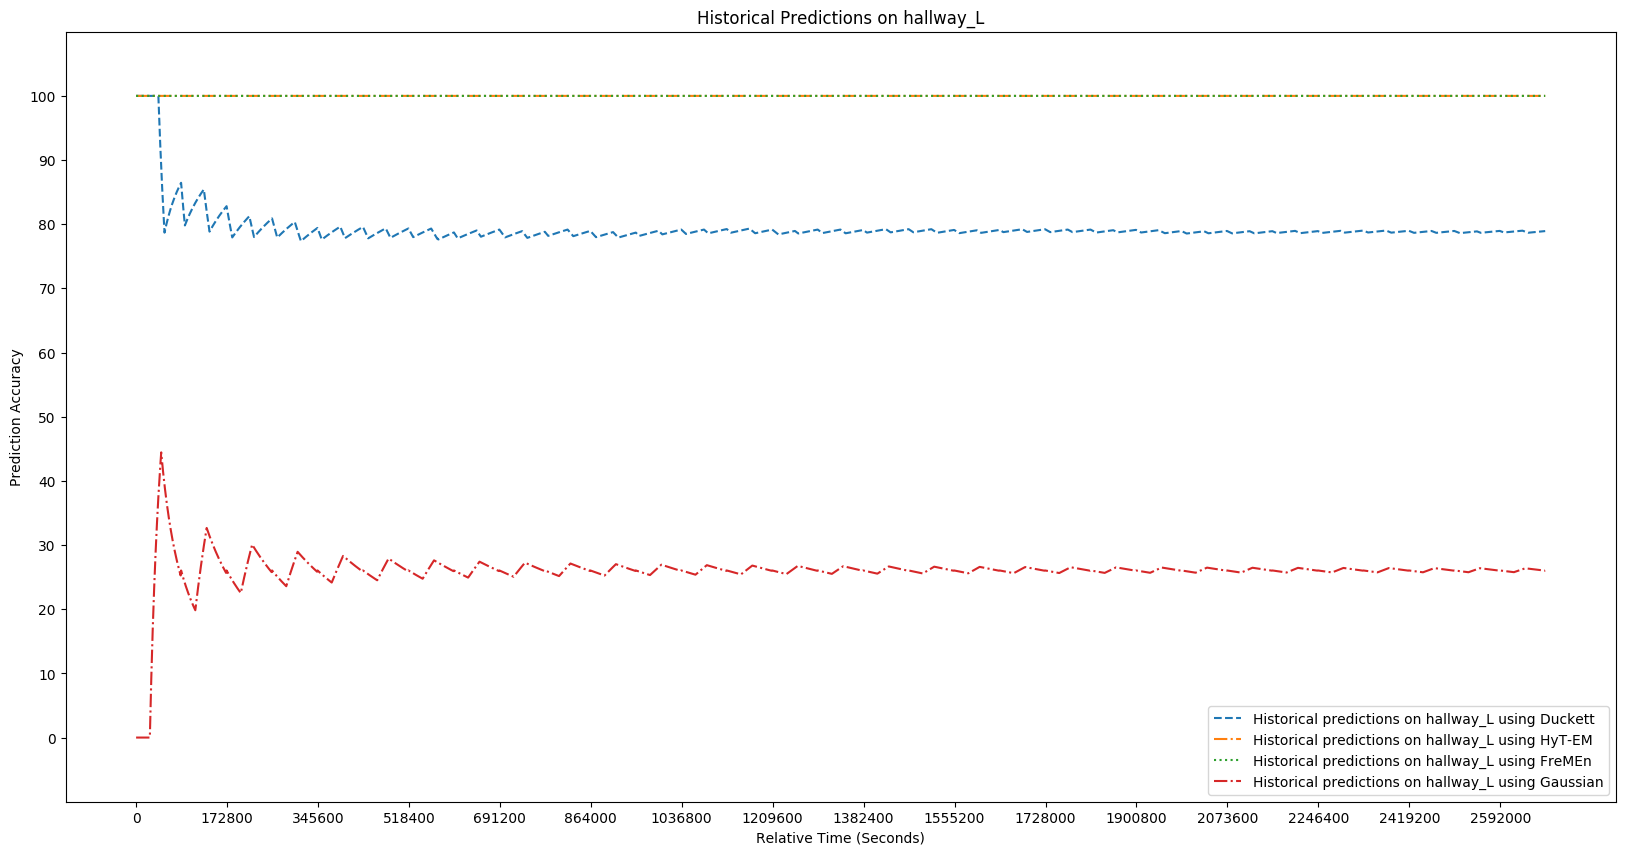
\includegraphics[width = 3in]{images/results/Historical_Predictions_on_hallway_L.png}} \\
  \end{tabular}
  \caption{Model Accuracy Over Time - Hallway Laundry}
\end{figure}\\ \\



\begin{figure}
  \begin{tabular}{cc}
    {\includegraphics[width = 3in]{images/results/Historical_hallway_M0_Duckett.png}} &
    {\includegraphics[width = 3in]{images/results/Historical_hallway_M0_FreMEn.png}} \\
    {\includegraphics[width = 3in]{images/results/Historical_hallway_M0_Gaussian.png}} &
    {\includegraphics[width = 3in]{images/results/Historical_hallway_M0_HyT-EM.png}} \\
  \end{tabular}
  \caption{Historical Recreations - Hallway Meal Section 0}
\end{figure}\\ \\

\begin{figure}
  \begin{tabular}{cc}
    {\includegraphics[width = 3in]{images/results/Future_hallway_M0_Duckett.png}} &
    {\includegraphics[width = 3in]{images/results/Future_hallway_M0_FreMEn.png}} \\
    {\includegraphics[width = 3in]{images/results/Future_hallway_M0_Gaussian.png}} &
    {\includegraphics[width = 3in]{images/results/Future_hallway_M0_HyT-EM.png}} \\
  \end{tabular}
  \caption{Future Predictions - Hallway Meal Section 0}
\end{figure}\\ \\

\begin{figure}
  \begin{tabular}{cc}
    {\includegraphics[width = 3in]{images/results/Future_Predictions_on_hallway_M0.png}} &
    {\includegraphics[width = 3in]{images/results/Historical_Predictions_on_hallway_M0.png}} \\
  \end{tabular}
  \caption{Model Accuracy Over Time - Hallway Meal Section 0}
\end{figure}\\ \\



\begin{figure}
  \begin{tabular}{cc}
    {\includegraphics[width = 3in]{images/results/Historical_hallway_M1_Duckett.png}} &
    {\includegraphics[width = 3in]{images/results/Historical_hallway_M1_FreMEn.png}} \\
    {\includegraphics[width = 3in]{images/results/Historical_hallway_M1_Gaussian.png}} &
    {\includegraphics[width = 3in]{images/results/Historical_hallway_M1_HyT-EM.png}} \\
  \end{tabular}
  \caption{Historical Recreations - Hallway Meal Section 1}
\end{figure}\\ \\

\begin{figure}
  \begin{tabular}{cc}
    {\includegraphics[width = 3in]{images/results/Future_hallway_M1_Duckett.png}} &
    {\includegraphics[width = 3in]{images/results/Future_hallway_M1_FreMEn.png}} \\
    {\includegraphics[width = 3in]{images/results/Future_hallway_M1_Gaussian.png}} &
    {\includegraphics[width = 3in]{images/results/Future_hallway_M1_HyT-EM.png}} \\
  \end{tabular}
  \caption{Future Predictions - Hallway Meal Section 1}
\end{figure}\\ \\

\begin{figure}
  \begin{tabular}{cc}
    {\includegraphics[width = 3in]{images/results/Future_Predictions_on_hallway_M1.png}} &
    {\includegraphics[width = 3in]{images/results/Historical_Predictions_on_hallway_M1.png}} \\
  \end{tabular}
  \caption{Model Accuracy Over Time - Hallway Meal Section 1}
\end{figure}\\ \\



\begin{figure}
  \begin{tabular}{cc}
    {\includegraphics[width = 3in]{images/results/Historical_hallway_T0_Duckett.png}} &
    {\includegraphics[width = 3in]{images/results/Historical_hallway_T0_FreMEn.png}} \\
    {\includegraphics[width = 3in]{images/results/Historical_hallway_T0_Gaussian.png}} &
    {\includegraphics[width = 3in]{images/results/Historical_hallway_T0_HyT-EM.png}} \\
  \end{tabular}
  \caption{Historical Recreations - Hallway Trash Section 0}
\end{figure}\\ \\

\begin{figure}
  \begin{tabular}{cc}
    {\includegraphics[width = 3in]{images/results/Future_hallway_T0_Duckett.png}} &
    {\includegraphics[width = 3in]{images/results/Future_hallway_T0_FreMEn.png}} \\
    {\includegraphics[width = 3in]{images/results/Future_hallway_T0_Gaussian.png}} &
    {\includegraphics[width = 3in]{images/results/Future_hallway_T0_HyT-EM.png}} \\
  \end{tabular}
  \caption{Future Predictions - Hallway Trash Section 0}
\end{figure}\\ \\

\begin{figure}
  \begin{tabular}{cc}
    {\includegraphics[width = 3in]{images/results/Future_Predictions_on_hallway_T0.png}} &
    {\includegraphics[width = 3in]{images/results/Historical_Predictions_on_hallway_T0.png}} \\
  \end{tabular}
  \caption{Model Accuracy Over Time - Hallway Trash Section 0}
\end{figure}\\ \\



\begin{figure}
  \begin{tabular}{cc}
    {\includegraphics[width = 3in]{images/results/Historical_hallway_T1_Duckett.png}} &
    {\includegraphics[width = 3in]{images/results/Historical_hallway_T1_FreMEn.png}} \\
    {\includegraphics[width = 3in]{images/results/Historical_hallway_T1_Gaussian.png}} &
    {\includegraphics[width = 3in]{images/results/Historical_hallway_T1_HyT-EM.png}} \\
  \end{tabular}
  \caption{Historical Recreations - Hallway Trash Section 1}
\end{figure}\\ \\

\begin{figure}
  \begin{tabular}{cc}
    {\includegraphics[width = 3in]{images/results/Future_hallway_T1_Duckett.png}} &
    {\includegraphics[width = 3in]{images/results/Future_hallway_T1_FreMEn.png}} \\
    {\includegraphics[width = 3in]{images/results/Future_hallway_T1_Gaussian.png}} &
    {\includegraphics[width = 3in]{images/results/Future_hallway_T1_HyT-EM.png}} \\
  \end{tabular}
  \caption{Future Predictions - Hallway Trash Section 1}
\end{figure}\\ \\

\begin{figure}
  \begin{tabular}{cc}
    {\includegraphics[width = 3in]{images/results/Future_Predictions_on_hallway_T1.png}} &
    {\includegraphics[width = 3in]{images/results/Historical_Predictions_on_hallway_T1.png}} \\
  \end{tabular}
  \caption{Model Accuracy Over Time - Hallway Trash Section 1}
\end{figure}\\ \\





\section{ Busy Elevators }


Duckett good at
\end{document}
